%================================
% note-setup-borderless.tex
% fenglielie@qq.com 2025-07-10
%================================
\documentclass{article}
\usepackage{amsmath,amsthm,amsfonts,amssymb}
\usepackage{mathtools}
\usepackage{mathrsfs}
\usepackage{bm}
\usepackage{extarrows}
\usepackage[a4paper, margin=1in]{geometry}
\usepackage{float}
\usepackage{indentfirst}
\usepackage{anyfontsize}
\usepackage{booktabs,multirow,multicol}
\usepackage[shortlabels,inline]{enumitem}
\usepackage{appendix}

\usepackage[dvipsnames]{xcolor}
\usepackage{graphicx}
\graphicspath{
    {./figure/}{./figures/}{./image/}{./images/}{./graphic/}{./graphics/}{./picture/}{./pictures/}
}
\usepackage{subcaption}

\usepackage[ruled,linesnumbered,noline]{algorithm2e}
\usepackage{listings}
\lstdefinestyle{simpleStyle}{
    basicstyle=\ttfamily\small,
    breaklines=true,
    keywordstyle=\color{blue},
    identifierstyle=\color{black},
    stringstyle=\color{violet},
    commentstyle=\color[RGB]{34,139,34},
    showstringspaces=false,
    numbers=left,
    numbersep=2em,
    numberstyle=\footnotesize,
    frame=single,
    framesep=1em,
}
\lstset{style=simpleStyle}

\usepackage[colorlinks=true, linkcolor=, urlcolor=magenta, citecolor=violet]{hyperref}

\renewcommand*{\proofname}{\normalfont\bfseries Proof}

\usepackage{thmtools}

%% define environments

\declaretheorem[style=plain, name=Theorem, numbered=yes, numberwithin=section]{theorem}
\declaretheorem[style=plain, name=Theorem, numbered=no]{theorem*}

\declaretheorem[style=plain, name=Proposition, numbered=yes, sibling=theorem]{proposition}
\declaretheorem[style=plain, name=Proposition, numbered=no]{proposition*}

\declaretheorem[style=plain, name=Corollary, numbered=yes, sibling=theorem]{corollary}
\declaretheorem[style=plain, name=Corollary, numbered=no]{corollary*}

\declaretheorem[style=plain, name=Lemma, numbered=yes, sibling=theorem]{lemma}
\declaretheorem[style=plain, name=Lemma, numbered=no]{lemma*}

\declaretheorem[style=plain, name=Claim, numbered=yes, sibling=theorem]{claim}
\declaretheorem[style=plain, name=Claim, numbered=no]{claim*}

\declaretheorem[style=definition, name=Definition, numbered=yes, numberwithin=section]{definition}
\declaretheorem[style=definition, name=Definition, numbered=no]{definition*}

\declaretheorem[style=definition, name=Example, numbered=yes, numberwithin=section]{example}
\declaretheorem[style=definition, name=Example, numbered=no]{example*}

\declaretheorem[style=definition, name=Problem, numbered=yes, numberwithin=section]{problem}
\declaretheorem[style=definition, name=Problem, numbered=no]{problem*}

\declaretheorem[style=remark, name=Remark, numbered=yes, numberwithin=section]{remark}
\declaretheorem[style=remark, name=Remark, numbered=no]{remark*}

\declaretheorem[style=remark, name=Note, numbered=yes, numberwithin=section]{note}
\declaretheorem[style=remark, name=Note, numbered=no]{note*}

\declaretheoremstyle[headfont=\bfseries, bodyfont=\normalfont, spaceabove=3pt, spacebelow=3pt, qed=\ensuremath{\square}]{solutionstyle}

\declaretheorem[style=solutionstyle, name=Solution, numbered=yes, numberwithin=section]{solution}
\declaretheorem[style=solutionstyle, name=Solution, numbered=no]{solution*}

\usepackage[most]{tcolorbox}

\newcommand{\newtcbenvironment}[2]{
    \tcolorboxenvironment{#1}{#2, enhanced, breakable, sharp corners, boxrule=0pt, colframe=white}
    \tcolorboxenvironment{#1*}{#2, enhanced, breakable, rounded corners, boxrule=0pt, colframe=white}
}

%% define styles

\newtcbenvironment{theorem}{colframe=RoyalPurple, colback=RoyalPurple!8}
\newtcbenvironment{proposition}{colframe=RoyalPurple, colback=RoyalPurple!8}
\newtcbenvironment{corollary}{colframe=NavyBlue, colback=SkyBlue!8}
\newtcbenvironment{lemma}{colframe=NavyBlue, colback=SkyBlue!8}
\newtcbenvironment{claim}{colframe=NavyBlue, colback=SkyBlue!8}

\newtcbenvironment{definition}{colframe=ForestGreen, colback=ForestGreen!5}
\newtcbenvironment{example}{colframe=RawSienna, colback=RawSienna!5}
\newtcbenvironment{problem}{colframe=WildStrawberry!30, colback=WildStrawberry!5}

%Exercise Environment
\newtheorem{exercise}{Exercise}

\title{MAT4033 Differential Geometry}
\author{Zihan Ke}

\begin{document}
\maketitle
\newpage
\tableofcontents
\newpage
\section*{Foreward}
The note is the typed notes for the course MAT4033 Differential Geometry,in CUHKSZ, taught by Professor Hou. The course mainly focus on curves and surfaces in the 3-dimensional Euclidean Space. We explore the concepts like Gaussian Curvature, Geodesics, etc. The course is wrapped up by the Gauss-Bonnet Theorem.

A special Remark on the Exercise: all the exercises appear in the note are the exercises left by Professot Hou during each class. The exerises usually asked you to check something for yourselves. It is beneficial to go thorough them if you are preparing for the exam.
\newpage
\section*{Introduction}
\noindent In this course we study curves and surfaces in $\mathbb{R^3}$

What are we interested in?
\begin{itemize}
    \item How we decribe a curve?
    \\ use the parametrization: $\alpha:I \to \mathbb{R}^3 $
    \item How much information can we get from $\alpha$?
    \\ length, curvature, torsion
    \item If we know the curvature of a curve of evrey point, can we describe the curve?
    \item Some "global" problems: Suppose we have a closed curve in $\mathbb{R}^3$ of a given length, what is the largest possible area bounded by the curve?
    \item How do we describe a surface? More precisely, what kind of surface should we study?
    \item For a regular surface, how can we study the area and curvature of them?
    \item What is the "shortest" between two points of a surface?
    \item What is the relationship between geometry and topology on surfaces? (Gauss-Bonnet Theorem)
\end{itemize}
\newpage
\section{Local Theory of Curves}

\begin{definition}[Regular Curve]
    A parameterized differentiable curve $\alpha: I \to \mathbb{R}^3$ is called \textbf{regular} if $\alpha'(t) \neq 0$ for all $t \in I$.
\end{definition}

\begin{proposition}
    Let $\alpha:[a,b]\to \mathbb{R}^3$ be a continuously differentiable curve. Let $P=\{a=t_0<t_1<\cdots <t_n=b\}$ be a partition of $[a,b]$.
    Let $l(\alpha,P):=\sum_{i=0}^{n-1} |\alpha(t_{i+1})-\alpha(t_{i})|$. Then the arc length is given by:
    \[ \int_a^b |\alpha'(t)| dt = \sup_P \{ l(\alpha,P) \} \]
\end{proposition}

\begin{proof}
    For any partition $P$, by the Fundamental Theorem of Calculus, $\alpha(t_{i+1}) - \alpha(t_i) = \int_{t_i}^{t_{i+1}} \alpha'(t) dt$.
    By the triangle inequality for integrals, $|\alpha(t_{i+1}) - \alpha(t_i)| \le \int_{t_i}^{t_{i+1}} |\alpha'(t)| dt$.
    Summing over $i$, we get $l(\alpha, P) \le \int_a^b |\alpha'(t)| dt$. Thus, $\sup_P l(\alpha, P) \le \int_a^b |\alpha'(t)| dt$.
    
    Conversely, since $\alpha'$ is continuous on a closed interval, it is uniformly continuous. For any $\epsilon > 0$, there exists $\delta > 0$ such that $|s-t| < \delta \implies |\alpha'(s) - \alpha'(t)| < \epsilon$.
    Choose a partition $P$ with mesh size less than $\delta$. Then:
    \[ \left| \sum |\alpha(t_{i+1}) - \alpha(t_i)| - \int_a^b |\alpha'(t)| dt \right| \le \sum \int_{t_i}^{t_{i+1}} |\alpha'(t) - \frac{\alpha(t_{i+1})-\alpha(t_i)}{\Delta t_i}| dt \]
    By the Mean Value Theorem applied to components (or direct estimation using uniform continuity), the difference inside the integral can be bounded by $\epsilon$. Thus the Riemann sum approximates the integral arbitrarily well.
\end{proof}

\begin{proposition}[Length is Invariant under Reparametrization]
   Given a differentiable curve $\alpha:[a,b]\to \mathbb{R}^3$ and a reparametrization map $g:[c,d] \to [a,b]$ with $g(c)=a, g(d)=b$ (orientation preserving) or $g(c)=b, g(d)=a$ (orientation reversing), let $\beta = \alpha \circ g$. Then:
   \[ \int_a^b |\alpha'(t)| dt = \int_c^d |\beta'(u)| du \]
\end{proposition}

\begin{proof}
    Let $t = g(u)$. By the Chain Rule, $\beta'(u) = (\alpha \circ g)'(u) = \alpha'(g(u)) g'(u)$.
    Therefore, $|\beta'(u)| = |\alpha'(g(u))| |g'(u)|$.
    
    If $g$ is orientation preserving ($g' > 0$), then $|g'(u)| = g'(u)$. By the change of variables formula for integrals:
    \[ \int_c^d |\beta'(u)| du = \int_c^d |\alpha'(g(u))| g'(u) du = \int_{g(c)}^{g(d)} |\alpha'(t)| dt = \int_a^b |\alpha'(t)| dt. \]
    If $g$ is orientation reversing ($g' < 0$), then $|g'(u)| = -g'(u)$.
    \[ \int_c^d |\beta'(u)| du = -\int_c^d |\alpha'(g(u))| g'(u) du = -\int_{b}^{a} |\alpha'(t)| dt = \int_a^b |\alpha'(t)| dt. \]
\end{proof}

\begin{remark}
    The cusp (e.g., $\alpha(t) = (t^3, t^2)$ at $t=0$) is not a regular curve since $\alpha'(0)=0$. Regularity ensures the curve has a well-defined tangent line everywhere.
\end{remark}

\subsection{Reparametrization}

\begin{definition}
    A \textbf{reparametrization} of a curve $\alpha: I \to \mathbb{R}^3$ is a bijective map $g: J \to I$ such that $g$ is smooth and $g^{-1}$ is smooth (which implies $g'(u) \neq 0$ everywhere). The new curve is $\beta = \alpha \circ g$.
\end{definition}

\begin{proposition}
    If $\alpha$ is a regular curve and $g$ is a reparametrization, then $\beta = \alpha \circ g$ is also regular.
\end{proposition}

\begin{proof}
    By the Chain Rule, $\beta'(u) = \alpha'(g(u)) g'(u)$.
    Since $\alpha$ is regular, $\alpha'(g(u)) \neq 0$. Since $g$ is a diffeomorphism, $g'(u) \neq 0$.
    The product of a non-zero vector and a non-zero scalar is a non-zero vector. Thus $\beta'(u) \neq 0$.
\end{proof}

\begin{proposition}
    The unit tangent vector is invariant (up to sign) under reparametrization.
\end{proposition}

\begin{proof}
    Let $T_\alpha(t) = \frac{\alpha'(t)}{|\alpha'(t)|}$. Let $\beta(u) = \alpha(g(u))$.
    \[ T_\beta(u) = \frac{\beta'(u)}{|\beta'(u)|} = \frac{\alpha'(g(u)) g'(u)}{|\alpha'(g(u)) g'(u)|} = \frac{\alpha'(g(u))}{|\alpha'(g(u))|} \frac{g'(u)}{|g'(u)|} = \text{sgn}(g') T_\alpha(g(u)) \]
    Thus, the tangent vector direction depends only on the geometric trace, not the speed.
\end{proof}

\subsection{Arc-length Parametrization}

To develop the theory of curves, it is convenient to eliminate the dependency on "speed" and parameterize by distance traveled.

\begin{definition}[Arc-length function]
    Let $\alpha: [a,b] \to \mathbb{R}^3$ be regular. Fix $t_0 \in [a,b]$. The arc-length function $s(t)$ is:
    \[ s(t) = \int_{t_0}^t |\alpha'(\tau)| d\tau \]
\end{definition}

\begin{lemma}
    The map $s: [a,b] \to [0, L]$ is a valid reparametrization map.
\end{lemma}

\begin{proof}
    Since $\alpha$ is regular, $|\alpha'(t)| > 0$. By the Fundamental Theorem of Calculus, $\frac{ds}{dt} = |\alpha'(t)| > 0$.
    Since the derivative is strictly positive, $s(t)$ is strictly increasing and therefore bijective. Since $s'(t) \neq 0$, by the Inverse Function Theorem, the inverse map $t(s)$ is also differentiable.
\end{proof}

\begin{definition}
    A curve $\beta(s)$ is \textbf{parameterized by arc-length} (p.a.l.) if $|\beta'(s)| = 1$ for all $s$.
\end{definition}

\begin{proposition}
    If we reparametrize $\alpha$ by the inverse of its arc-length function, the resulting curve is p.a.l.
\end{proposition}

\begin{proof}
    Let $t = t(s)$ be the inverse of $s(t)$. Let $\beta(s) = \alpha(t(s))$.
    \[ \beta'(s) = \alpha'(t(s)) \frac{dt}{ds} = \alpha'(t) \frac{1}{s'(t)} = \alpha'(t) \frac{1}{|\alpha'(t)|} \]
    Therefore, $|\beta'(s)| = \frac{|\alpha'(t)|}{|\alpha'(t)|} = 1$.
\end{proof}

\subsection{Frenet Frames of Plane Curves}

Assume $\alpha: I \to \mathbb{R}^2$ is a plane curve parameterized by arc length $s$.
We have the unit tangent $t(s) = \alpha'(s)$. Since $|t(s)|^2 = 1$, differentiating gives $2\langle t'(s), t(s) \rangle = 0$, so $t'(s) \perp t(s)$.

\begin{definition}
    Define the \textbf{normal vector} $n(s)$ by rotating $t(s)$ by $90^\circ$ counter-clockwise (i.e., applying the complex map $J(x,y) = (-y, x)$).
    $\{t(s), n(s)\}$ is a positively oriented orthonormal basis.
    Since $t'(s) \perp t(s)$, it must be parallel to $n(s)$. We define the \textbf{curvature} $k(s)$ by:
    \[ t'(s) = k(s) n(s) \]
\end{definition}

\begin{proposition}[Formula for arbitrary parametrization]
    Let $\alpha(t)$ be a regular plane curve (not necessarily p.a.l.). The curvature is:
    \[ k(t) = \frac{\det(\alpha'(t), \alpha''(t))}{|\alpha'(t)|^3} \]
\end{proposition}

\begin{proof}
    Let $s$ be the arc-length parameter and $v = \frac{ds}{dt} = |\alpha'(t)|$. We have $\alpha'(t) = v t(s)$.
    Differentiating again with respect to $t$ (using chain rule $\frac{d}{dt} = v \frac{d}{ds}$):
    \[ \alpha''(t) = \frac{d}{dt}(v t(s)) = v' t(s) + v \frac{d}{dt}(t(s)) = v' t(s) + v^2 t'(s) \]
    Using the definition $t'(s) = k n(s)$, we get:
    \[ \alpha''(t) = v' t(s) + k v^2 n(s) \]
    Now compute the determinant (in $\mathbb{R}^2$, $\det(a,b)$ is the signed area of the parallelogram):
    \[ \det(\alpha', \alpha'') = \det(v t, v' t + k v^2 n) = v v' \det(t, t) + k v^3 \det(t, n) \]
    Since $\det(t,t)=0$ and $\det(t,n)=1$ (orthonormal basis):
    \[ \det(\alpha', \alpha'') = k v^3 = k |\alpha'|^3 \]
    Rearranging gives $k = \frac{\det(\alpha', \alpha'')}{|\alpha'|^3}$.
\end{proof}

\begin{theorem}[Fundamental Theorem of Plane Curves]
    Given a smooth function $k: I \to \mathbb{R}$, there exists a p.a.l. curve $\alpha: I \to \mathbb{R}^2$, unique up to rigid motion, having $k(s)$ as its curvature.
\end{theorem}

\begin{proof}
    Let $\theta(s)$ be the angle of the tangent vector. We must have $\theta'(s) = k(s)$.
    Define $\theta(s) = \int_{s_0}^s k(u) du + \theta_0$.
    Define $\alpha(s) = (\int_{s_0}^s \cos\theta(u) du + x_0, \int_{s_0}^s \sin\theta(u) du + y_0)$.
    Then $\alpha'(s) = (\cos\theta, \sin\theta)$, which is unit length.
    $t'(s) = (-\sin\theta \cdot \theta', \cos\theta \cdot \theta') = \theta' n(s) = k(s) n(s)$.
    Thus $\alpha$ has the desired curvature.
    Uniqueness follows from the uniqueness of ODE solutions (or simple integration as shown above).
\end{proof}

\subsection{Space Curves}

Let $\alpha(s)$ be a p.a.l. curve in $\mathbb{R}^3$. $t(s) = \alpha'(s)$.
Since $t' \perp t$, if $t'(s) \neq 0$, we define the \textbf{curvature} $\kappa(s) = |t'(s)|$ and the \textbf{principal normal} $n(s) = \frac{t'(s)}{\kappa(s)}$.
Define the \textbf{binormal} $b(s) = t(s) \times n(s)$.

\begin{proposition}[Frenet-Serret Formulas]
    \[
    \frac{d}{ds} \begin{pmatrix} t \\ n \\ b \end{pmatrix} = \begin{pmatrix} 0 & \kappa & 0 \\ -\kappa & 0 & -\tau \\ 0 & \tau & 0 \end{pmatrix} \begin{pmatrix} t \\ n \\ b \end{pmatrix}
    \]
\end{proposition}

\begin{proof}
    1. By definition, $t' = \kappa n$.
    2. Since $b = t \times n$, $b' = t' \times n + t \times n' = \kappa n \times n + t \times n' = t \times n'$.
    Thus $b' \perp t$. Also $|b|=1 \implies b' \perp b$. So $b'$ must be parallel to $n$.
    Define $\tau(s)$ such that $b'(s) = -\tau(s) n(s)$. (The sign is convention).
    3. Since $\{t,n,b\}$ is orthonormal, $n = b \times t$.
    $n' = b' \times t + b \times t' = -\tau n \times t + b \times \kappa n = -\tau (-b) + \kappa (-t) = -\kappa t + \tau b$.
\end{proof}

Now we present some applications of Frenet-Serret Formulas.

\begin{example}
    Let $\alpha$ be a regular curve with $\kappa > 0$. Then $\alpha$ is a plane curve if and only if $\tau \equiv 0$.
\end{example}

\begin{proof}
    ($\Rightarrow$) Suppose $\alpha$ lies in a plane defined by $v \cdot (x - x_0) = 0$ ($v$ is constant unit normal).
    Differentiating $\alpha(s) \cdot v = \text{const}$ gives $t(s) \cdot v = 0$.
    Differentiating again: $t' \cdot v = \kappa n \cdot v = 0$. Since $\kappa \neq 0$, $n \cdot v = 0$.
    Since $t \perp v$ and $n \perp v$, $b = t \times n$ must be parallel to $v$.
    Thus $b(s) = \pm v = \text{const}$. Hence $b'(s) = 0$. By Frenet formulas, $-\tau n = 0 \implies \tau = 0$.

    ($\Leftarrow$) Suppose $\tau \equiv 0$. Then $b'(s) = 0$, so $b(s) = b_0$ (constant).
    Consider the function $f(s) = \langle \alpha(s) - \alpha(0), b_0 \rangle$.
    $f'(s) = \langle t(s), b_0 \rangle$. Since $b_0 = t \times n$, $b_0 \perp t$, so $f'(s) = 0$.
    Thus $f(s) = 0$ for all $s$. $\alpha(s)$ lies in the plane passing through $\alpha(0)$ with normal $b_0$.
\end{proof}

\begin{example}
    $\alpha$ is a straight line if and only if all tangent lines pass through a fixed point $x_0$.
\end{example}

\begin{proof}
    ($\Rightarrow$) Trivial.
    ($\Leftarrow$) Assume $\alpha(s) + \lambda(s) t(s) = x_0$ for some scalar function $\lambda(s)$.
    Differentiate: $t(s) + \lambda'(s) t(s) + \lambda(s) \kappa(s) n(s) = 0$.
    Taking inner product with $n(s)$: $\lambda(s) \kappa(s) = 0$.
    If $\lambda(s) = 0$, then $\alpha(s) = x_0$ (not a regular curve). Thus $\lambda \neq 0$, implying $\kappa(s) = 0$.
    $\kappa = 0 \implies t'(s) = 0 \implies t(s) = \text{const} \implies \alpha(s)$ is a line.
\end{proof}

\begin{example}
    Let $\alpha$ be a curve such that every normal plane passes through a fixed point $x_0$. Then $\alpha$ lies on a sphere.
\end{example}

\begin{proof}
    The normal plane at $s$ is spanned by $n(s), b(s)$. The condition implies $x_0 - \alpha(s)$ lies in this plane.
    Thus $x_0 - \alpha(s) \perp t(s)$.
    $\langle \alpha(s) - x_0, t(s) \rangle = 0$.
    Consider $f(s) = |\alpha(s) - x_0|^2 = \langle \alpha(s) - x_0, \alpha(s) - x_0 \rangle$.
    $f'(s) = 2 \langle \alpha'(s), \alpha(s) - x_0 \rangle = 2 \langle t(s), \alpha(s) - x_0 \rangle = 0$.
    Thus $|\alpha(s) - x_0|^2$ is constant, so $\alpha$ lies on a sphere centered at $x_0$.
\end{proof}
\begin{exercise}
    Prove the above three examples (it is left as an exeercise in class, I include the proof here).
\end{exercise}
\subsection{Fundamental Theorem of Space Curves}

\begin{theorem}
    Given smooth functions $\kappa(s) > 0$ and $\tau(s)$, there exists a space curve $\alpha(s)$, unique up to rigid motion, with curvature $\kappa$ and torsion $\tau$.
\end{theorem}

\begin{proof}
    \textbf{Existence:} Consider the system of linear ODEs for a $3 \times 3$ matrix function $F(s) = (t(s) | n(s) | b(s))$:
    \[ F'(s) = F(s) \begin{pmatrix} 0 & -\kappa & 0 \\ \kappa & 0 & -\tau \\ 0 & \tau & 0 \end{pmatrix} \]
    (Note: This is the transpose of the usual form if vectors are columns).
    By the Existence Theorem for ODEs, there exists a unique solution $F(s)$ with $F(0) = I$.
    We must show the columns remain orthonormal. Let $M = F^T F$.
    $M' = (F')^T F + F^T F' = (F A)^T F + F^T (F A) = A^T (F^T F) + (F^T F) A = A^T M + M A$.
    Since $A$ is skew-symmetric ($A^T = -A$), $M(s) = I$ is a solution to this differential equation ($I' = 0$ and $A^T I + I A = -A + A = 0$). By uniqueness, $M(s) = I$ for all $s$.
    Thus $\{t,n,b\}$ are orthonormal.
    Define $\alpha(s) = \int_0^s t(u) du$. Then $\alpha' = t$, so it is p.a.l.
    $t' = \kappa n$ (matches curvature).
    $n' = -\kappa t + \tau b$ (matches torsion).

    \textbf{Uniqueness:} Let $\alpha, \tilde{\alpha}$ be two such curves. Align their initial positions and frames by a rigid motion. Let $f(s) = |t - \tilde{t}|^2 + |n - \tilde{n}|^2 + |b - \tilde{b}|^2$.
    Using the Frenet equations, one shows $f'(s) = 0$. Since $f(0)=0$, $f(s) \equiv 0$.
    Thus $t(s) = \tilde{t}(s)$, so $\alpha(s) = \tilde{\alpha}(s)$ after integration.
\end{proof}
\newpage
\section{Global Theory of Curves}
In this section we would like to study the theory of plane curves globally. 

An important question in geometry is the following. Suppose we know the local property of a curve, can we say some thing about the global properties of it?

\subsection{Hopf's Umlaufsatz}
\begin{definition}
    The rotation index of $\alpha:I\to \mathbb{R}^3$ with period is given by \[\frac{\theta(a)-\theta(0)}{2\pi}=\frac{1}{2\pi}\int_0^a\theta'(s)ds\]. where $\theta(s)$ is defined by $t(s)=(\cos(\theta(s)),\sin(\theta(s)))$.
\end{definition}

\begin{theorem}[Hopf's Umlaufsatz]
Suppose $\alpha$ is a simple closed curve, then its rotation index must be equal to $\pm 1$. Moreover, since we have $\theta'(s)=\kappa(s)$, we have $\int\kappa(s)ds=\pm2\pi$.    
\end{theorem}
\begin{proof}
Let the curve $\alpha: [0, L] \to \mathbb{R}^2$ be a simple closed curve parameterized by arc length $s$. The unit tangent vector is $T(s) = \alpha'(s)$, and its angle with a fixed axis is $\theta(s)$. The total curvature is the net change in this angle, $\theta(L) - \theta(0)$. Since the curve is closed, $T(L) = T(0)$, which implies $\theta(L) - \theta(0) = 2\pi $ for some integer $n$. We will show that $n = \pm 1$.

As suggested by the proof sketch, we introduce the unit secant vector field, which maps two points on the curve to the unit vector connecting them:
\[ u(s_1, s_2) = \frac{\alpha(s_2) - \alpha(s_1)}{||\alpha(s_2) - \alpha(s_1)||} \]
This map is smooth provided $s_1 \neq s_2$, which is guaranteed for a simple curve. Let $\phi(s_1, s_2)$ be the angle of this secant vector.

This angle function is defined on the domain $[0, L] \times [0, L]$ excluding the diagonal. We consider the triangular region $D = \{(s_1, s_2) \mid 0 \le s_1 \le s_2 \le L\}$. Since $\phi$ is a smooth, well-defined function on the interior of $D$, its exterior derivative $d\phi$ is an exact 1-form. By Green's theorem (or Stokes' theorem for forms), the integral of $d\phi$ around the boundary $\partial D$ must be zero, provided we handle the singular diagonal edge properly.
\[ \oint_{\partial D} d\phi = 0 \]
The boundary $\partial D$ consists of three segments. A careful limiting argument shows that the integral of $d\phi$ over the boundary is the sum of the changes in angle along the limiting paths.
\begin{enumerate}
    \item \textbf{The diagonal path ($s_1=s_2$):} As $s_2 \to s_1$, the secant vector $u(s_1, s_2)$ limits to the tangent vector $T(s_1)$. Thus, the angle $\phi(s,s)$ corresponds to the tangent angle $\theta(s)$. The change in angle along this path is the total curvature: $\Delta\phi_{diag} = \theta(L) - \theta(0)$.

    \item \textbf{The `start' path ($s_1=0$):} This path corresponds to the secant vector $u(0,s_2)$ from the fixed starting point $\alpha(0)$ to a moving point $\alpha(s_2)$. Let the total change in its angle be $\Delta\phi_{start} = \phi(0,L) - \phi(0,0)$.

    \item \textbf{The `end' path ($s_2=L$):} This path corresponds to the secant vector $u(s_1,L)$ from a moving point $\alpha(s_1)$ to the fixed end point $\alpha(L)=\alpha(0)$. This vector is the opposite of the `start' vector: $u(s_1,L) = -u(0,s_1)$. Thus their angles are related by $\phi_{end}(s_1) = \phi_{start}(s_1) \pm \pi$. The total change in angle along this path is $\Delta\phi_{end} = \Delta\phi_{start}$.
\end{enumerate}

The relationship between these changes in angle, derived from the boundary integral being zero, is:
\[ \theta(L) - \theta(0) = \Delta\phi_{start} + \Delta\phi_{end} \]
Substituting $\Delta\phi_{end} = \Delta\phi_{start}$, we get:
\[ \theta(L) - \theta(0) = 2 \Delta\phi_{start} \]
Now we must evaluate $\Delta\phi_{start}$. This quantity represents the total rotation of the secant line anchored at $\alpha(0)$ as its other end traverses the entire curve. Since the curve $\alpha$ is simple and closed, it encloses a region. The secant vector starts in the direction of the tangent $T(0)$ and, as it sweeps through the interior of the curve, ends by pointing in the opposite direction, $-T(0)$. This corresponds to a net rotation of exactly half a circle. Therefore, the change in angle is:
\[ \Delta\phi_{start} = \pm\pi \]
Substituting this result into our equation gives the final result:
\[ \int_0^L \kappa(s) \, ds = \theta(L) - \theta(0) = 2(\pm \pi) = \pm 2\pi \]
This shows that the rotation index $n$ must be either $+1$ or $-1$.
\end{proof}

% For the Hopf's Umlaufsatz illustration
\begin{figure}[h!] % [h!] tries to place the figure "here"
    \centering % Centers the image
    \includegraphics[width=0.4\textwidth,height=0.3\textwidth]{hopf_secants.pdf} % Adjust width as needed
    \caption{Illustration of secant vectors from a fixed point on a closed curve,
             visualizing the $\Delta\phi_{start}$ component in the proof of Hopf's Umlaufsatz.}
    \label{fig:hopf_secants} % Label for cross-referencing
\end{figure}

\begin{remark}
    The theorem can be viewed as a 1-dimensional version of Gauss-Bonnet Formula.
\end{remark}

\subsection{Isoperimetric Inequality}

\begin{theorem}[Isoperimetric Inequality]
    Let $\alpha$ be a simple closed plane curve. Let A be the area bounded by curves, then $L^2\geq 4\pi A$
\end{theorem}
\begin{proof}
The proof compares the area of the given curve $\mathcal{C}$ to that of a circle $\mathcal{S}^1$ by relating their parametrizations.

\paragraph{Step 1: The Setup.}
Let $\mathcal{C}$ be a simple closed curve of length $L$ enclosing area $A$. We can parameterize $\mathcal{C}$ by arc length, $\gamma(t) = (x(t), y(t))$ for $t \in [0, L]$. A key property of this parametrization is that the tangent vector has unit length:
\[ (x'(t))^2 + (y'(t))^2 = 1 \]
We construct a circle $\mathcal{S}^1$ of an arbitrary radius $r$ centered at the origin. We then define a new curve, $\beta(t) = (x(t), \tilde{y}(t))$, which traces this circle using the same x-coordinate as $\gamma(t)$. To ensure $\beta(t)$ remains on the circle, we must have $\tilde{y}(t) = \pm\sqrt{r^2 - x(t)^2}$.
% For the Isoperimetric Inequality illustration
\begin{figure}[h!]
    \centering
    \includegraphics[width=0.5\textwidth]{isoperimetric_proof.png} % Adjust width
    \caption{Geometric construction for the proof of the Isoperimetric Inequality.
             Curve C (red) and constructed circle S\textsuperscript{1} (blue) sharing x-coordinates.}
    \label{fig:isoperimetric_proof}
\end{figure}

\paragraph{Step 2: Combining the Area Formulas.}
Using Green's Theorem, we can express the areas as line integrals:
\begin{itemize}
    \item The area of $\mathcal{C}$ is $A = \int_0^L x(t)y'(t) \, dt$.
    \item The area of the circle $\mathcal{S}^1$ is $\pi r^2 = -\int_0^L \tilde{y}(t)x'(t) \, dt$.
\end{itemize}
Adding these two expressions for area yields:
\[ A + \pi r^2 = \int_0^L \left( x(t)y'(t) - \tilde{y}(t)x'(t) \right) \, dt \]

\paragraph{Step 3: Applying the Cauchy-Schwarz Inequality.}
The integrand can be interpreted as the dot product of two vectors, $\mathbf{v}_1(t) = (x(t), -\tilde{y}(t))$ and $\mathbf{v}_2(t) = (y'(t), x'(t))$. We apply the Cauchy-Schwarz inequality for integrals, which states $\int \mathbf{v}_1 \cdot \mathbf{v}_2 \, dt \le \int ||\mathbf{v}_1|| \, ||\mathbf{v}_2|| \, dt$.
\[ A + \pi r^2 \le \int_0^L \sqrt{x(t)^2 + (-\tilde{y}(t))^2} \cdot \sqrt{y'(t)^2 + x'(t)^2} \, dt \]
The terms in the integral simplify significantly:
\begin{itemize}
    \item Since $\beta(t)$ is on the circle, $\sqrt{x(t)^2 + \tilde{y}(t)^2} = \sqrt{r^2} = r$.
    \item Since $\gamma(t)$ is parameterized by arc length, $\sqrt{y'(t)^2 + x'(t)^2} = 1$.
\end{itemize}
Substituting these back, the inequality becomes:
\[ A + \pi r^2 \le \int_0^L r \cdot 1 \, dt = rL \]

\paragraph{Step 4: Finding the Optimal Bound.}
We have derived the relation $A \le rL - \pi r^2$, which must hold for any choice of $r > 0$. To find the tightest possible bound for $A$, we find the value of $r$ that maximizes the function $f(r) = rL - \pi r^2$. Taking the derivative with respect to $r$ and setting it to zero gives:
\[ f'(r) = L - 2\pi r = 0 \implies r = \frac{L}{2\pi} \]
This is the radius of a circle with perimeter $L$. Substituting this optimal radius back into our inequality yields:
\begin{align*}
    A &\le \left(\frac{L}{2\pi}\right)L - \pi\left(\frac{L}{2\pi}\right)^2 \\
    A &\le \frac{L^2}{2\pi} - \pi\left(\frac{L^2}{4\pi^2}\right) \\
    A &\le \frac{L^2}{2\pi} - \frac{L^2}{4\pi} \\
    A &\le \frac{L^2}{4\pi}
\end{align*}
Rearranging this gives the isoperimetric inequality: $4\pi A \le L^2$.

\paragraph{The Equality Case.}
Equality holds if the Cauchy-Schwarz inequality becomes an equality, which occurs if and only if the vectors $\mathbf{v}_1(t)$ and $\mathbf{v}_2(t)$ are parallel for all $t$. This means $\mathbf{v}_1(t) = k \, \mathbf{v}_2(t)$ for some scalar $k$. The magnitudes must also be equal, so $|k| \cdot ||\mathbf{v}_2|| = ||\mathbf{v}_1||$, which gives $|k| \cdot 1 = r$, so $k = \pm r$.

This implies that $x(t) = \pm r y'(t)$ and $-\tilde{y}(t) = \pm r x'(t)$. For the parametrizations to match, the original curve $\gamma(t)$ must itself be a circle of radius $r$. Since the optimal radius was $r = L/(2\pi)$, equality holds if and only if $\mathcal{C}$ is a circle.
\end{proof}

\subsection{Four vertex Theorem (Covered in Tutorial)}

We begin by defining the key concepts required for the theorem and its proof. Let $\gamma(t) = (x(t), y(t))$ be a regular plane curve.

\begin{definition}[Signed Curvature]
For a regular plane curve $\gamma(t)$ parameterized by arc length $s$, its velocity vector is $\mathbf{v}(s) = \gamma'(s)$ and its acceleration is $\mathbf{a}(s) = \gamma''(s)$. The signed curvature, $k_s(s)$, is defined by the relation $\mathbf{a}(s) = k_s(s) R_{90}(\mathbf{v}(s))$, where $R_{90}$ is a 90-degree counter-clockwise rotation. For a general parameter $t$, the curvature equations are:
\begin{align}
    x''(t) &= -k_s(t)y'(t) \\
    y''(t) &= k_s(t)x'(t)
\end{align}
\end{definition}

\begin{definition}[Vertex]
A point $\gamma(t)$ on the trace of a regular plane curve is called a \textbf{vertex} if the signed curvature function $k_s$ has a local maximum or a local minimum at $t$.
\end{definition}

\begin{definition}[Convex Curve]
A simple closed plane curve is called \textbf{convex} if its trace lies entirely on one closed side of each of its tangent lines.
\end{definition}

Now we state the four vertex theorem.

\begin{theorem}[The Four Vertex Theorem]
\label{thm:four_vertex}
Every simple closed plane curve has at least four vertices.
\end{theorem}

\noindent
\textit{Note: The following proof addresses the special case where the curve is convex.}

The proof relies on the following geometric property of convex curves.

\begin{lemma}
\label{lem:convexity}
Let $C$ be the trace of a simple closed convex plane curve, and let $L$ be a line. If $L$ intersects $C$ in at least three points, then $C$ must contain the entire line segment of $L$ between any pair of these points.
\end{lemma}

\noindent
A direct consequence is that if a line is not part of the curve, it can intersect a convex curve at most twice.


\begin{proof}[Proof of Theorem \ref{thm:four_vertex} for Convex Curves]
The proof is by contradiction.

\paragraph{Step 1: The Contradiction Hypothesis.}
Assume there exists a simple, closed, convex curve $\gamma$ with fewer than four vertices. Since the continuous curvature function $k_s$ on a closed curve must attain a global maximum and a global minimum, the curve must have at least two vertices. As local maxima and minima must alternate, the number of vertices must be even. Therefore, our assumption implies that $\gamma$ has exactly two vertices:
\begin{itemize}
    \item A point $p$ where $k_s$ attains its global maximum.
    \item A point $q$ where $k_s$ attains its global minimum.
\end{itemize}

\paragraph{Step 2: Geometric Setup.}
Let $L$ be the line passing through the points $p$ and $q$. By Lemma \ref{lem:convexity}, since the curve is convex and not a line segment, $L$ can intersect the curve only at points $p$ and $q$.

We can apply a rigid motion (translation and rotation) to the curve to simplify our coordinate system without changing its geometric properties. We set up the coordinates such that:
\begin{itemize}
    \item The point $p$ is at the origin, $p=(0,0)$.
    \item The line $L$ is the x-axis.
    \item The point $q$ is on the positive x-axis, $q=(a,0)$ for some $a>0$.
\end{itemize}
Let the curve be parameterized by $\gamma(t) = (x(t), y(t))$ for $t \in [0, l]$.

\paragraph{Step 3: Analysis of the Functions.}
From our setup, the entire curve lies on one side of the x-axis. We can assume without loss of generality that $y(t) \ge 0$ for all $t \in [0,l]$.
Furthermore, for a positively oriented (counter-clockwise) simple closed convex curve, the signed curvature $k_s(t)$ is strictly positive.

Therefore, the product of these two functions, $y(t)k_s(t)$, must be non-negative for all $t$, and it is only zero at the points $p$ and $q$.

\paragraph{Step 4: The Contradiction.}
We analyze the integral of the product $y(t)k_s(t)$ over the entire curve.
\begin{enumerate}
    \item \textbf{The integral must be positive.} Since $y(t)k_s(t) \ge 0$ for all $t$ and is not identically zero, its integral must be strictly positive:
    $$ \int_0^l y(t)k_s(t) \, dt > 0 $$

    \item \textbf{The integral must be zero.} However, as stated in the textbook's argument, integrating by parts and using the curvature equations from (1) and (2) shows that the integral is zero. A key part of such a derivation involves using the fact that for a closed curve, the integral of an exact derivative is zero. For example, using equation (2), $y''(t) = k_s(t)x'(t)$, we know:
    $$ \int_0^l k_s(t)x'(t) \, dt = \int_0^l y''(t) \, dt = \left[ y'(t) \right]_0^l = 0 $$
    The textbook asserts that a similar line of reasoning (though not fully detailed) leads to the conclusion that our original integral is zero.
\end{enumerate}

We have reached a contradiction: the integral cannot be both strictly positive and equal to zero. Thus, our initial assumption that the curve has fewer than four vertices must be false. This completes the proof.
\end{proof}
\newpage
\section{Local Theory of Surfaces}
\subsection{Introduction}
\begin{definition}
A \textbf{parameterized surface} is a function $X: U \subseteq \mathbb{R}^2 \rightarrow \mathbb{R}^3$ where $Z$ is differentiable. We say $Z$ is \textbf{regular} if the Jacobian matrix
\[
dX= \begin{pmatrix}
\frac{\partial x}{\partial u} & \frac{\partial x}{\partial v} \\
\frac{\partial y}{\partial u} &\frac{\partial y}{\partial v} \\
\frac{\partial z}{\partial u} &\frac{\partial z}{\partial v}
\end{pmatrix}
\]
has rank 2 for all points in $U$. In coordinates:
\[
X(u,v) = (x(u,v), y(u,v), z(u,v))
\]
Equivalently, $Z: U \subseteq \mathbb{R}^2 \rightarrow \mathbb{R}^3$ is an embedding. The image $Z(U)$ is called the \textbf{trace} of $Z$.
\end{definition}

\begin{remark}
For regular curves $\alpha: I \rightarrow \mathbb{R}^3$, we require $\alpha' \neq 0$. For surfaces, the analogous condition is that the differential has full rank.
\end{remark}

\begin{example}
    Consider the parameterization:
\[
X: (0,2\pi) \times (0,\pi) \rightarrow \mathbb{R}^3
\]
\[
X(\theta, \varphi) = (r\cos\theta\sin\varphi, r\sin\theta\sin\varphi, r\cos\varphi)
\]


This parameterization $Z$ is regular because
\[
\frac{\partial X}{\partial \theta} \times \frac{\partial X}{\partial \varphi} \neq 0
\]
and the Jacobian matrix has rank 2.

\end{example}
As in the case of curves. We wish to parametrize a surface to do Calculus on surfaces. Of course we need two variables rather than 1 variable in the curve case.
\begin{remark}[Problem of the parametrized surface]
The above example of ${S}^2$ reveals that in order to develop a unified theory for studying surfaces, it is necessary to use more than one coordinate patch. Now we would like to introduce the concept of regular surface.  
\end{remark}
\begin{definition}
A subset $S \subset \mathbb{R}^3$ is a \textbf{regular surface} if for every point $p \in S$, there exists a neighborhood $V \subset \mathbb{R}^3$ of $p$ (which can be taken as an open ball centered at $p$ with radius $r > 0$) and a map $X: U \rightarrow V \cap S$ where $U \subset \mathbb{R}^2$ is open and connected, such that:

\begin{enumerate}
    \item $X$ is differentiable: 
    \[
    X(u,v) = (x(u,v), y(u,v), z(u,v)), \quad (u,v) \in U
    \]
    has partial derivatives of all orders.
    
    \item $X$ is bijective with continuous inverse $X^{-1}$, i.e., $X$ is a homeomorphism.
    
    \item (Regularity) For $q \in U$ with $X(q) = p$, the Jacobian matrix
    \[
    dX_q = \begin{pmatrix}
    \frac{\partial x}{\partial u} & \frac{\partial x}{\partial v} \\
    \frac{\partial y}{\partial u} & \frac{\partial y}{\partial v} \\
    \frac{\partial z}{\partial u} & \frac{\partial z}{\partial v}
    \end{pmatrix}
    \]
    has rank 2 for all $q \in U$.
\end{enumerate}
\end{definition}

\begin{remark}
    Conditions (2) and (3) together guarantee that $X$ is an embedding from $U$ to $S$, ensuring the existence of a tangent plane at each point of $S$. This is analogous to the requirement $\alpha' \neq 0$ for regular curves.
\end{remark}

\begin{example}
Let $S^2 = \{(x,y,z) \in \mathbb{R}^3 \mid x^2 + y^2 + z^2 = 1\}$ be the unit sphere. We can cover $S^2$ using 6 coordinate patches. For example, let
\[
U = \{(x,y) \in \mathbb{R}^2 \mid x^2 + y^2 < 1\}
\]
and define the coordinate patch for the upper hemisphere:
\[
X(x,y) = \left(x, y, \sqrt{1 - x^2 - y^2}\right), \quad (x,y) \in U
\]
And then we can do the same for other coordinates.
\end{example}

\begin{example}
    Suppose $f: U \subseteq \mathbb{R}^2 \rightarrow \mathbb{R}$ is a smooth map. Then the graph of $f$ defined as
\[
S = \operatorname{graph}(f) = \{(x, y, z) \in \mathbb{R}^3 \mid (x, y) \in U, z = f(x, y)\}
\]
is a regular surface.\newline
\noindent \underline{Homework}: Check the graph is indeed a regular surface.
\end{example}

The above example shows that graph is a regular surface, and indeed the converse is in some sense true. Every regular surface is Locally a graph.

\begin{proposition}
Any regular surface $S$ is locally a graph.
\end{proposition}

\begin{proof}
Let $p \in S$ be any point and let $X: U \rightarrow V \cap S$ be the coordinate patch given in the definition of regular surfaces, with $X(q) = p$. By the regularity condition, the differential
\[
dX_q = \begin{pmatrix}
\frac{\partial X}{\partial u} & \frac{\partial X}{\partial v}
\end{pmatrix}
\]
has rank 2. This means that among the three possible $2 \times 2$ Jacobian matrices:
\[
\begin{pmatrix}
\frac{\partial x}{\partial u} & \frac{\partial x}{\partial v} \\
\frac{\partial y}{\partial u} & \frac{\partial y}{\partial v}
\end{pmatrix}, \quad
\begin{pmatrix}
\frac{\partial x}{\partial u} & \frac{\partial x}{\partial v} \\
\frac{\partial z}{\partial u} & \frac{\partial z}{\partial v}
\end{pmatrix}, \quad
\begin{pmatrix}
\frac{\partial y}{\partial u} & \frac{\partial y}{\partial v} \\
\frac{\partial z}{\partial u} & \frac{\partial z}{\partial v}
\end{pmatrix}
\]
at least one has nonzero determinant.

Without loss of generality, assume the first Jacobian matrix has nonzero determinant. Then by the inverse function theorem, the projection
\[
\pi \circ X: (u,v) \mapsto (x(u,v), y(u,v))
\]
has a differentiable inverse in some neighborhood of $q$.

Let $g = (\pi \circ X)^{-1}$ be this inverse mapping, which sends $(x,y) \mapsto (u(x,y), v(x,y))$. Then we have
\[(x,y)\to (u,v)\to (x,y,z(x(u,v),y(u,v)))\]
By the formulas we see that indeed it is locally a graph.
\end{proof}
\begin{remark}
    The above proof is a routine technique to apply the inverse function/implicit function theorem in geometry.
\end{remark}

\begin{example}
Let $f: \mathbb{R}^3 \rightarrow \mathbb{R}$ be a smooth map and $a \in \mathbb{R}$ be such that for all $p \in f^{-1}(a)$, the differential $(df)_p \neq 0$ (i.e., $a$ is a regular value of $f$). Then $f^{-1}(a) \subset \mathbb{R}^3$ is a regular surface.
\begin{proof}
For any $p \in f^{-1}(a)$, suppose without loss of generality that $\left(\frac{\partial f}{\partial z}\right)_p \neq 0$.

Define the function $F: \mathbb{R}^3 \rightarrow \mathbb{R}$ by:
\[
F(x) = f(x) - a
\]
Then $F(p) = 0$.

Since $\left(\frac{\partial F}{\partial z}\right)_p = \left(\frac{\partial f}{\partial z}\right)_p \neq 0$, by the implicit function theorem, there exists a smooth function $g: U \subset \mathbb{R}^2 \rightarrow \mathbb{R}$ such that:
\[
F(u, g(u)) = 0 \quad \forall u \in U
\]
where $U$ is an open neighborhood in $\mathbb{R}^2$.

This means we can express a neighborhood of $p \in f^{-1}(a)$ as:
\[
W = \{(u, g(u)) \mid u \in U\}, \quad \text{with } p = (u_0, g(u_0))
\]

Therefore, there exists a neighborhood $V$ such that:
\[
V \cap f^{-1}(a) = \{(x, y, z) \mid (x, y) \in U, z = g(x, y)\}
\]

This shows that every point $p \in f^{-1}(a)$ is locally a graph, hence by the previous proposition about graphs of functions being regular surfaces, $f^{-1}(a)$ is a regular surface.
\end{proof}
\end{example}

\begin{example}
Consider the ellipsoid defined by the equation:
\[
\frac{x^2}{a^2} + \frac{y^2}{b^2} + \frac{z^2}{c^2} = 1
\]
where $a, b, c > 0$ are constants.
\begin{proof}
Define the function $F: \mathbb{R}^3 \rightarrow \mathbb{R}$ by:
\[
F(x, y, z) = \frac{x^2}{a^2} + \frac{y^2}{b^2} + \frac{z^2}{c^2} - 1
\]

Then:
\begin{enumerate}
    \item $F$ is obviously differentiable (in fact, smooth) on $\mathbb{R}^3$
    
    \item The differential of $F$ is given by:
    \[
    dF = \left( \frac{\partial F}{\partial x}, \frac{\partial F}{\partial y}, \frac{\partial F}{\partial z} \right) = \left( \frac{2x}{a^2}, \frac{2y}{b^2}, \frac{2z}{c^2} \right)
    \]
    
    \item For any point $w = (w_1, w_2, w_3) \in F^{-1}(0)$ (i.e., on the ellipsoid), we have:
    \[
    dF(w) = \left( \frac{2w_1}{a^2}, \frac{2w_2}{b^2}, \frac{2w_3}{c^2} \right)
    \]
    
    Since $w$ lies on the ellipsoid, at least one coordinate must be nonzero, hence $dF(w) \neq 0$. Therefore, 0 is a regular value of $F$.
\end{enumerate}

By the regular value theorem, $F^{-1}(0)$ is a regular surface.
\end{proof}
\end{example}

\begin{remark}
    For the sphere $S^2$,it is possible to cover the surface using only 2 coordinate patches. See Streographic Peojection.
\end{remark}
\begin{example}[Stereographic Projection]
    See Homework.
\end{example}
\subsection{Change of Coordinates}
Recall that for curves, we may have different parametrizations. The same holds for regular surfaces. We say that two parametrizations describe the same surface even if they use different coordinate systems.

\begin{proposition}
Let $p \in S$ be a point in the image of two parametrizations:
\[
X: U \rightarrow S \quad \text{and} \quad Y: V \rightarrow S
\]
Let $W = X(U) \cap Y(V)$ be the overlapping region. Then the transition map
\[
\varphi = X^{-1} \circ Y: Y^{-1}(W) \rightarrow X^{-1}(W)
\]
defined by $(u,v) \mapsto (u',v')$ is a diffeomorphism.
\end{proposition}

\begin{proof}
Since both $X$ and $Y$ are regular parametrizations, they are homeomorphisms onto their images and their differentials have full rank. Therefore:

1. $\varphi$ is well-defined as a map between open subsets of $\mathbb{R}^2$

2. $\varphi$ is a homeomorphism because it is the composition of homeomorphisms

3. $\varphi$ is differentiable because both $X$ and $Y$ are differentiable and regular

4. The inverse $\varphi^{-1} = Y^{-1} \circ X$ is similarly differentiable

The Jacobian matrix of the transition map is given by:
\[
d\varphi = \begin{pmatrix}
\frac{\partial u'}{\partial u} & \frac{\partial u'}{\partial v} \\
\frac{\partial v'}{\partial u} & \frac{\partial v'}{\partial v}
\end{pmatrix}
\]
This matrix is invertible everywhere because $\varphi$ is a diffeomorphism.
\end{proof}
\begin{remark}
This property is fundamental in manifold theory. It ensures that geometric properties defined using different coordinate systems are consistent. The transition maps allow us to define a smooth structure on the surface $S$ by specifying how different coordinate patches relate to each other.
This is exactly the property we aim to generalize in the theory of smooth manifolds, where we use charts and transition maps to define the smooth structure.
\end{remark}

\subsection{Tangent plane}
\begin{definition}
Let $\mathbf{x}: U \to \text{VAS}$ be a coordinate patch of a regular surface at a $\text{pt } \mathbf{x}(p) = p \in S$. Then the tangent plane at $p \in S$ is defined as
\[
T_p S = \text{Im} \left( (\mathrm{d}\mathbf{x})_p \right) = \text{span} \left\{ \frac{\partial \mathbf{x}}{\partial u} (p), \frac{\partial \mathbf{x}}{\partial v} (p) \right\}.
\]
\end{definition}

\begin{definition}
The normal vector of a $\text{pt } p$ on a coordinate patch $\mathbf{x}: U \to \text{VAS}$ is defined as
\[
N(p) = \frac{\frac{\partial \mathbf{x}}{\partial u} \times \frac{\partial \mathbf{x}}{\partial v}}{\left\| \frac{\partial \mathbf{x}}{\partial u} \times \frac{\partial \mathbf{x}}{\partial v} \right\|} \quad (p)
\]
\end{definition}

\noindent \underline{Problem:} 
although the tangent plane is well-defined, but $N(p)$ may be affected by our choice of coordinates. (the sign).

\begin{definition}
A tangent vector at $p \in S$ is the tangent vector $\alpha'(0)$ of a regular curve $\alpha: (-\varepsilon, \varepsilon) \to S \subseteq \mathbb{R}^3$ with $\alpha(0) = p$.
\end{definition}

\begin{proposition}
The set of tangent vectors at $p \in S$ is precisely equal to $T_p S$.
\end{proposition}

\begin{proof}
Let $\alpha: (-\varepsilon, \varepsilon) \to S$ be regular with $\alpha(0)=p$.
Recall that $\exists \ V$ of $p \in S$ such that by restricting $\text{VAS}$ to $V \cap S$, we have $\mathbf{y}: U' \to V \cap S$
such that $\mathbf{y}(u', v') = (u', v', f(u', v'))$
or $(u', g(u', v'), v')$ (locally a graph).

we look at the first case. w.l.o.g. by making $\varepsilon$ small enough.
assume $\alpha(-\varepsilon, \varepsilon) \subseteq V \cap S$.

Let $\beta$ be given by $\beta: (-\varepsilon, \varepsilon) \to U' \subseteq \mathbb{R}^2$
where $\mathbf{y}^{-1}$ is differentiable. ($\mathbf{y}^{-1}$ is just the projection map)
Then $\alpha = \mathbf{y} \circ \beta = \mathbf{x} \circ (\mathbf{x}^{-1} \circ \mathbf{y} \circ \beta)$

we've seen in prop that $\mathbf{x}^{-1} \circ \mathbf{y}$ is differentiable
so $\alpha'(0) = (\mathrm{d}\mathbf{x})_q \cdot (\mathrm{d}(\mathbf{x}^{-1} \circ \mathbf{y} \circ \beta)) (0)$
\[
= \left( \frac{\partial \mathbf{x}}{\partial u}, \frac{\partial \mathbf{x}}{\partial v} \right)_q \begin{pmatrix} a \\ b \end{pmatrix}
\]
$\Rightarrow \alpha'(0) \in T_p S$.
We've just seen that $\alpha'(0) \in T_p S$.

Now we must to see $\mathbf{w} \in T_p S \Rightarrow \mathbf{w} = \alpha'(0)$ for some $\alpha$.
Suppose $\mathbf{w} = \left( \frac{\partial \mathbf{x}}{\partial u} (p), \frac{\partial \mathbf{x}}{\partial v} (p) \right) \begin{pmatrix} a \\ b \end{pmatrix} \in T_p S$.
Then let $\beta: (-\varepsilon, \varepsilon) \to U$ by $\beta(t) = p + t \begin{pmatrix} a \\ b \end{pmatrix}$.
and $\alpha = \mathbf{x} \circ \beta$. Then $\alpha(0) = \mathbf{x}(\beta(0)) = \mathbf{x}(p) = p$.
$\alpha'(0) = (\mathrm{d}\mathbf{x})_p \cdot \mathrm{d}\beta_0 = \left( \frac{\partial \mathbf{x}}{\partial u}, \frac{\partial \mathbf{x}}{\partial v} \right) \begin{pmatrix} a \\ b \end{pmatrix} \in T_p S$.
\end{proof}
\begin{example}
    Suppose $f: \mathbb{R}^3 \to \mathbb{R}$ smooth. $S = f^{-1}(a)$.
Let $\alpha: (-\varepsilon, \varepsilon) \to S$ with $\alpha(0)=p$. Then
\[
f(\alpha(t)) = f(x(t), y(t), z(t)) = a.
\]
Differentiating with respect to $t$:
\[
\Rightarrow (\mathrm{d}f)_p \cdot (\mathrm{d}\alpha)_0 = 0.
\]
\[
\Rightarrow (\mathrm{d}f)_p \cdot \alpha'(0) = 0.
\]
$\Rightarrow (\mathrm{d}f)_p$ is always normal to $T_p S$.
\end{example}

\noindent \underline{Question:} we define $N(p)$ on a coordinate patch. can we choose coordinates patch appropriately so that $N: S \to \mathbb{R}^3$ is a smooth function?

\begin{remark}
    When we move from local to global, it is always determined by the "topology" property.
\end{remark}

\subsection{First Fundamental Form }
After defining the tangent plane, we wil study the inner product structure so that we can compute the area of the surface.

\begin{definition}
    Let $V$ be a vector space. We study $\langle \cdot, \cdot \rangle : V \times V \to \mathbb{R}$ an inner product if it satisfies the following:
\begin{enumerate}
    \item $\langle \mathbf{v}, \mathbf{w} \rangle = \langle \mathbf{w}, \mathbf{v} \rangle$ (symmetric).
    \item $\langle a\mathbf{v}_1 + b\mathbf{v}_2, \mathbf{w} \rangle = a \langle \mathbf{v}_1, \mathbf{w} \rangle + b \langle \mathbf{v}_2, \mathbf{w} \rangle$ (linearity).
    \item $\langle \mathbf{v}, \mathbf{v} \rangle \ge 0 \quad \forall \mathbf{v} \in V$. equality holds if and only if $\mathbf{v}=\mathbf{0}$.
\end{enumerate}
\end{definition}

\begin{definition}
The quadratic form corresponding to an inner product is a map $q: V \to \mathbb{R}$ defined by
\[
\mathbf{v} \to \langle \mathbf{v}, \mathbf{v} \rangle.
\]
\end{definition}

\begin{definition}
The \textbf{First Fundamental Form} of $S$ is given by the quadratic form $I_p(\mathbf{v}) = \langle \mathbf{v}, \mathbf{v} \rangle$ for $\mathbf{v} \in T_p S$.
\end{definition}
In order to understand $I_p$ better, we need to choose a basis of $T_p S$ and express $I_p$ using matrices and vectors.

Let $\mathbf{x}: U \to \text{VAS}$ be a coordinate patch with $\mathbf{x}(p)=p$.
Then $\mathcal{B} = \left\{ \mathbf{x}_u = \frac{\partial \mathbf{x}}{\partial u} (p), \mathbf{x}_v = \frac{\partial \mathbf{x}}{\partial v} (p) \right\}$
\begin{align*}
\text{with } E_p &= \langle \mathbf{x}_u, \mathbf{x}_u \rangle_p \\
F_p &= \langle \mathbf{x}_u, \mathbf{x}_v \rangle_p \\
G_p &= \langle \mathbf{x}_v, \mathbf{x}_v \rangle_p
\end{align*}
(We drop the subscript $p$ if it does not cause confusion)

Then for all $\mathbf{v}$, $I_p(\mathbf{v}) = (a, b) \begin{pmatrix} E & F \\ F & G \end{pmatrix} \begin{pmatrix} a \\ b \end{pmatrix}$.

More precisely, $\langle \mathbf{v}, \mathbf{w} \rangle_p = (a, b) \begin{pmatrix} E & F \\ F & G \end{pmatrix} \begin{pmatrix} c \\ d \end{pmatrix}$, where $\mathbf{v} = a \mathbf{x}_u + b \mathbf{x}_v$ and $\mathbf{w} = c \mathbf{x}_u + d \mathbf{x}_v$.

Therefore, in a coordinate patch $\text{IFF}$ refers to $\begin{pmatrix} E & F \\ F & G \end{pmatrix}$.

\begin{example}
\begin{enumerate}
    \item \textbf{Cylinder:}
    \[
    \mathbf{x}(u, v) = (\cos u, \sin u, v)
    \]
    \[
    \mathbf{x}_u = (-\sin u, \cos u, 0)
    \]
    \[
    \mathbf{x}_v = (0, 0, 1)
    \]
    $E = \langle \mathbf{x}_u, \mathbf{x}_u \rangle = 1. \quad F = 0. \quad G = 1.$
    \[
    \Rightarrow I_p = \begin{pmatrix} E & F \\ F & G \end{pmatrix} = \begin{pmatrix} 1 & 0 \\ 0 & 1 \end{pmatrix}
    \]

    \item \textbf{Plane:}
    \[
    \mathbf{x}(u, v) = \mathbf{x}_0 + u \mathbf{w}_1 + v \mathbf{w}_2
    \]
    (Assuming $\mathbf{w}_1$ and $\mathbf{w}_2$ are orthonormal, $\langle \mathbf{w}_i, \mathbf{w}_j \rangle = \delta_{ij}$)
    \[
    I_p = \begin{pmatrix} 1 & 0 \\ 0 & 1 \end{pmatrix}
    \]

    \item
    \[
    \mathbf{x}(u, v) = (u, v, \sqrt{1-u^2-v^2})
    \]
    \[
    \mathbf{x}_u = \left( 1, 0, \frac{-u}{\sqrt{1-u^2-v^2}} \right), \quad \mathbf{x}_v = \left( 0, 1, \frac{-v}{\sqrt{1-u^2-v^2}} \right)
    \]
    \[
    I_p = \begin{pmatrix}
        \frac{1-v^2}{1-u^2-v^2} & \frac{uv}{1-u^2-v^2} \\
        \frac{uv}{1-u^2-v^2} & \frac{1-u^2}{1-u^2-v^2}
    \end{pmatrix}
    \]
    (Note: This is the IFF for the upper hemisphere in Cartesian coordinates.)
    $\mathbf{\tilde{x}}_\varphi = (-\sin \phi \sin \varphi, \sin \phi \cos \varphi, 0)$.
% IFF for the sphere in spherical coordinates, assuming u=\phi, v=\varphi
\[
I_p = \begin{pmatrix} 1 & 0 \\ 0 & \sin^2 \phi \end{pmatrix} \quad \text{different expression of } I_p \text{ for the same surface } S
\]
\end{enumerate}
\end{example}

\noindent \underline{Question:}
Suppose we have 2 parameterizations
\[
\mathbf{x}: U \to V \cap S, \quad \mathbf{\tilde{x}}: \tilde{U} \to V \cap S.
\]
Note that
\[
\begin{pmatrix} \tilde{E} & \tilde{F} \\ \tilde{F} & \tilde{G} \end{pmatrix} = \left( \frac{\partial \mathbf{\tilde{x}}}{\partial \tilde{u}}, \frac{\partial \mathbf{\tilde{x}}}{\partial \tilde{v}} \right)^T \begin{pmatrix} \frac{\partial \mathbf{\tilde{x}}}{\partial \tilde{u}} \\ \frac{\partial \mathbf{\tilde{x}}}{\partial \tilde{v}} \end{pmatrix}
= (\mathrm{d}\mathbf{\tilde{x}})^T \mathrm{d}\mathbf{\tilde{x}}.
\]
Suppose $\Psi = \mathbf{x}^{-1} \circ \mathbf{\tilde{x}}$ is the transition function
\[
\Psi(\tilde{u}, \tilde{v}) = (u(\tilde{u}, \tilde{v}), v(\tilde{u}, \tilde{v})).
\]
\[
\Rightarrow \mathbf{\tilde{x}} = \mathbf{x} \circ \Psi. \quad \text{so}
\]
\[
\mathrm{d}\mathbf{\tilde{x}} = \mathrm{d}\mathbf{x} \mathrm{d}\Psi, \quad \text{and hence}
\]
\begin{align*}
\begin{pmatrix} \tilde{E} & \tilde{F} \\ \tilde{F} & \tilde{G} \end{pmatrix} &= (\mathrm{d}\mathbf{x} \mathrm{d}\Psi)^T (\mathrm{d}\mathbf{x} \mathrm{d}\Psi) \\
&= (\mathrm{d}\Psi)^T (\mathrm{d}\mathbf{x})^T (\mathrm{d}\mathbf{x}) (\mathrm{d}\Psi) \\
&= (\mathrm{d}\Psi)^T \begin{pmatrix} E & F \\ F & G \end{pmatrix} (\mathrm{d}\Psi)
\end{align*}
composition by \textbf{Jacobian matrix}.

\begin{example} Back to the sphere example.
\[
\Psi(\phi, \varphi) = (\sin \phi \cos \varphi, \sin \phi \sin \varphi)
\]
$\mathrm{d}\Psi = \begin{pmatrix}
\cos\phi \cos\varphi & -\sin\phi \sin\varphi \\
\cos\phi \sin\varphi & \sin\phi \cos\varphi
\end{pmatrix}$
and
\[
(\mathrm{d}\Psi)^T \begin{pmatrix} E & F \\ F & G \end{pmatrix} \mathrm{d}\Psi = \begin{pmatrix} 1 & \mathbf{0} \\ \mathbf{0} & \sin^2 \phi \end{pmatrix}
\]
\end{example}

\begin{corollary}
\[
\sqrt{\tilde{E}\tilde{G}-\tilde{F}^2} = \sqrt{EG-F^2} \ \det \left( \frac{\partial (u, v)}{\partial (\tilde{u}, \tilde{v})} \right)
\]
\begin{remark}
    We are always working in the orientable cases.
\end{remark}
\end{corollary}

With the first fundamental form, we can compute arc-length, area, etc.

\begin{enumerate}
    \item Arc-length.
    $$L(\gamma) = \int_I |\gamma'(t)| \, dt$$
    $$\gamma'(t) = X_u(u, v) u'(t) + X_v(u, v) v'(t)$$
    $$= \int_I \sqrt{|X_u u'(t) + X_v v'(t)|^2} \, dt$$
    $$= \int_I \sqrt{E |u'(t)|^2 + 2F u'(t) v'(t) + G |v'(t)|^2} \, dt.$$
    (If we consider $\gamma$ a curve on $S$ then first fundamental form gives us \textbf{Advantage}: a way to determine the arc-length \textbf{intrinsically}.)

    We just need to know $\alpha(t) = (x(t), y(t))$ to compute the arc-length of $\alpha$.

    \item Area of Surface
    \begin{definition}
        Let $Z: U \to S \cap V$ be a coordinate patch of $S$, and $R \in S$ be such that $Z(U) = R$ for $U \subset \mathbb{R}^2$. Then the area of $R$ is given by
        $$\int_A |X_u \times X_v| \, du \, dv.$$
    \end{definition}
    Note that $|u \times w|^2 = |u|^2 |w|^2 - (u \cdot w)^2$.
    That is $|X_u \times X_v| = \sqrt{EG - F^2}$.

    What happens if we have $\tilde{Z}: \tilde{U} \to S \cap \tilde{V}$ and $Z(U) = \tilde{Z}(\tilde{U}) = R$?
    Note that
    $$\Psi = Z^{-1} \circ \tilde{Z}: \tilde{U} \to U$$
    $$\int_{\tilde{R}} \sqrt{\tilde{E} \tilde{G} - \tilde{F}^2} \, d\tilde{u} \, d\tilde{v} = \int_R \sqrt{E G - F^2} \left|\frac{\partial(u, v)}{\partial(\tilde{u}, \tilde{v})}\right| \, d\tilde{u} \, d\tilde{v}$$
\end{enumerate}

$$= \int_R \sqrt{EG - F^2} \, du \, dv.$$
$$ \implies \text{Area of } R \text{ is independent of the choice of coordinate patch.}$$

\begin{remark}
    \textbf{Recall}:
    \begin{itemize}
        \item First fundamental form ($\text{f.f.f}$): $I_p(w) = \langle w, w \rangle, w \in T_p S$.
        \item If $X: U \to V \cap S$, $w = a X_u + b X_v$, then $I_p(w) = (a \ b) \begin{pmatrix} E & F \\ F & G \end{pmatrix} \begin{pmatrix} a \\ b \end{pmatrix}$.
    \end{itemize}
\end{remark}

\section{Gauss Map and the Second Fundamental Form}

\textbf{Main Goal}: Define curvature of a surface.

Recall that in the case of curves:
$$\vec{T}'(t) = \kappa(t) \vec{N}(t) \quad \text{in the case of plane curve.}$$
$$\vec{N}'(t) = -\kappa(t) \vec{T}(t)$$

So curvature of a plane curve can be measured by the changes of tangent/normal vector.

If we want to do this on surface, one would like to study the change of normal vector.

\textbf{Difficulty 1:}\\
The normal vector $N_p = \frac{X_u \times X_v}{\|X_u \times X_v\|}(q)$ is defined only up to a sign.

On each parametrization, one has a "smooth" choice of $N(p)$.
So we have:
$$N: V \cap S \to S^2$$
$$p \mapsto N(p) = \frac{X_u \times X_v}{\|X_u \times X_v\|}(q)$$

\begin{remark}
    \textbf{However}
    The map may not be able to be extended to whole $S$.
    For example, we have a problem defining $N: S \to S^2$ on a M\"obius band.
    The problem is the \textbf{orientability of $S$}.
\end{remark}

\begin{definition}
    Let $f: S_1 \to S_2$ be a map between two regular surfaces.
    We say $f$ is \textbf{smooth} if $Z_2^{-1} \circ f \circ Z_1$ is smooth.
    The surface $S$ is \textbf{orientable} if there is a smooth map
    $$N: S \to S^2$$
    such that $N(p) \perp T_p S$ for all $p \in S$.
\end{definition}

\begin{example}
    \begin{enumerate}
        \item Suppose $S$ is covered by one coordinate patch $Z: U \to S$.
        For example, $(S \text{ is the graph of a function } f)$.
        Then $N_{(p)} = \frac{X_u \times X_v}{\|X_u \times X_v\|}(q)$.
        \item Suppose $S = f^{-1}(0)$ is defined by an equation, then we can take
        $$N_{(p)} = \frac{D f(p)}{\|D f(p)\|} = \frac{(\frac{\partial f}{\partial x}, \frac{\partial f}{\partial y}, \frac{\partial f}{\partial z})}{|(\frac{\partial f}{\partial x}, \frac{\partial f}{\partial y}, \frac{\partial f}{\partial z})|} (p)$$
    \end{enumerate}
\end{example}

\textbf{Difficulty 2:} \\
For curves, we have $n' = -\kappa t$. For surfaces, we have two degrees of freedom on $S$.
\subsection{Gauss Map}
\begin{definition}
    The map $N$ is called \textbf{Gauss Map} of $S$. $N$ is well-defined up to a sign.
\end{definition}

\begin{definition}
    (Differential)
    Let $f: S_1 \to S_2$ be a map. The \textbf{differential} of $f$ at $p$, $d f_p$, is a map from $T_p S_1$ to $T_{f(p)} S_2$, defined by
    $$d f_p (v) := (f \circ \alpha)'(0),$$
    where $\alpha: (-\varepsilon, \varepsilon) \to S_1$ such that $\alpha(0) = p$, $\alpha'(0) = v$.
\end{definition}

\begin{remark}
    One needs to check this definition is well-defined.
    \textbf{Hint}: Instead of using the definition that $f$ is smooth if $\psi \circ f \circ \varphi^{-1}$ is smooth, one may use the definition that $f$ is smooth on $S_1 \subset \mathbb{R}^3$, if $f = F|_{S_1}$, where $F: \mathbb{R}^3 \to \mathbb{R}^3$ is smooth. It's much easier and intuitive in our cases.
\end{remark}

Now we study $d N_p: T_p S_1 \to T_{N(p)} S^2 \simeq T_p S$.
Geometrically, $d N_p$ measures how $N(p)$ changes along any direction of $T_p S$.

\begin{remark}
    One way to compute $d N_p: T_p S \to T_{N(p)} S^2$ is the following. Let $Z(u, v)$ coordinate patch of $S$.

    \begin{center}
        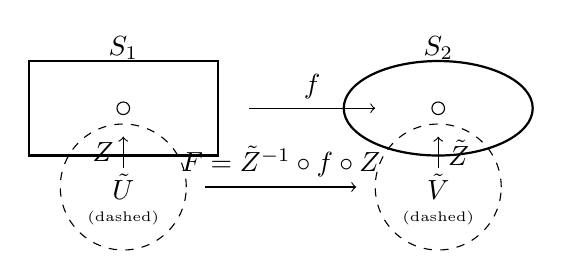
\begin{tikzpicture}[scale=0.8]
        \draw[thick] (0, 0) -- (3, 0) -- (3, 1.5) -- (0, 1.5) -- cycle;
        \node at (1.5, 1.7) {$S_1$};
        \draw (1.5, 0.75) circle (0.1);

        \draw[->] (3.5, 0.75) -- node[above] {$f$} (5.5, 0.75);

        \draw[thick] (6.5, 0.75) ellipse (1.5cm and 0.75cm);
        \node at (6.5, 1.7) {$S_2$};
        \draw (6.5, 0.75) circle (0.1);

        \node at (1.5, -0.5) {$\tilde{U}$};
        \node at (1.5, -1.0) {\tiny (dashed)};
        \draw[dashed] (1.5, -0.5) circle (1.0);
        \draw[->] (1.5, -0.2) -- node[left] {$Z$} (1.5, 0.3);

        \node at (6.5, -0.5) {$\tilde{V}$};
        \node at (6.5, -1.0) {\tiny (dashed)};
        \draw[dashed] (6.5, -0.5) circle (1.0);
        \draw[->] (6.5, -0.2) -- node[right] {$\tilde{Z}$} (6.5, 0.3);

        \draw[->] (2.8, -0.5) -- node[above] {$F = \tilde{Z}^{-1} \circ f \circ Z$} (5.2, -0.5);

        \end{tikzpicture}
    \end{center}

    If $w = a X_u + b X_v$,
    $$\begin{pmatrix} c \\ d \end{pmatrix} = \begin{pmatrix} \frac{\partial F_1}{\partial u} & \frac{\partial F_1}{\partial v} \\ \frac{\partial F_2}{\partial u} & \frac{\partial F_2}{\partial v} \end{pmatrix} \begin{pmatrix} a \\ b \end{pmatrix}$$
    $$(d f_p)(w) = c \tilde{Z}_{\tilde{u}} + d \tilde{Z}_{\tilde{v}}$$

    Consider $N \circ Z: U \to S^2$, by abuse of notation.
    Write this map as $N(u, v)$. ($\text{No } Z \text{ in that}$).

    To compute $d N_p$, take the "principal curve".
    $\beta(t) = (t, v_0)$. $\alpha = Z \circ \beta$. Has $\alpha'(0)=X_u$.
    Then $d N_p (X_u)$ is given by
    $$(N \circ \alpha)'(0) = (N \circ Z \circ \beta)'(0)$$
    $$= \frac{d}{d t} N(t, v_0)|_{t=0} = \frac{\partial N}{\partial u} = N_u.$$

    Similarly, $d N_p (X_v) = N_v = \frac{\partial N}{\partial v}$.

    Since $d N_p: T_p S \to T_{N(p)} S^2$ is a linear transformation
\end{remark}
% Uncertainty: The diagram illustrates $f: S_1 \to S_2$ and $F$ being the map between the parameter domains $\tilde{U}$ and $\tilde{V}$. However, the text immediately following the diagram relates to the differential $d f_p$, while the rest of the text focuses on the Gauss Map $N$. The first part of the remark seems to set up the general differential of a map $f$ (which is $d f_p$), while the second part is calculating $d N_p$ specifically. I've transcribed the content faithfully, including the diagram setup for the general differential.

And $\{X_u, X_v\}$ forms a basis of $T_p S$, one can get from
$$\begin{cases} d N_p (X_u) = N_u \\ d N_p (X_v) = N_v \end{cases}$$
Moreover, $\langle N, N \rangle = 1$, so differentiating yields $\langle d N, N \rangle = 0$.
$$\implies \langle N_u, N \rangle = 0 \implies N_u \in T_p S.$$
$$\implies \langle N_v, N \rangle = 0 \implies N_v \in T_p S.$$

$$\implies d N_p: T_p S \to T_p S.$$

\begin{example}
    Here are some concrete examples.
    \begin{enumerate}
        \item $S$ is a plane, i.e. $Z(u, v) = X_0 + u W_1 + v W_2$.
        $$X_u = W_1, \quad X_v = W_2$$
        $$\implies N(u, v) = \frac{X_u \times X_v}{\|X_u \times X_v\|} = \text{ constant.}$$
        $$\implies N_u = N_v = 0. \quad \text{i.e. } d N_p \text{ is the zero map.}$$

        \item Sphere $S^2$: $Z(u, v) = (u, v, \sqrt{1-u^2-v^2})$.
        $$X_u = \left(1, 0, \frac{-u}{\sqrt{1-u^2-v^2}}\right)$$
        $$X_v = \left(0, 1, \frac{-v}{\sqrt{1-u^2-v^2}}\right)$$
        $$N(u, v) = (u, v, \sqrt{1-u^2-v^2})$$
        $$N_u = X_u, \quad N_v = X_v$$
        $$\text{i.e. } d N_p (X_u) = X_u$$
        $$\text{i.e. } d N_p (X_v) = X_v$$
        Hence $d N_p$ is the \textbf{identity map}.
    \item $Z(u, v) = (u, v, u^2 - v^2)$.
    $$X_u = (1, 0, 2u), \quad X_v = (0, 1, -2v).$$
    $$N(u, v) = \left( \frac{-2u}{\sqrt{1 + 4u^2 + 4v^2}}, \frac{2v}{\sqrt{1 + 4u^2 + 4v^2}}, \frac{1}{\sqrt{1 + 4u^2 + 4v^2}} \right).$$

    Let $p = (0, 0, 0)$. ($u=0, v=0$).
    $$X_u|_p = (1, 0, 0), \quad X_v|_p = (0, 1, 0).$$
    $$N_u|_p = (-2, 0, 0), \quad N_v|_p = (0, 2, 0).$$
    $$d N_p (X_u) = N_u|_p = -2 X_u|_p, \quad d N_p (X_v) = N_v|_p = 2 X_v|_p.$$
    \end{enumerate}
\end{example}

\begin{proposition}
    The linear operator $d N_p$ is a \textbf{self-adjoint operator} with respect to the inner-product.
\end{proposition}

\begin{remark}
    In the finite-dimensional case, $A^* = A$. $\text{ker} \, A = (\text{Im} \, A^*)^\perp$. $\text{ker} \, A^* = (\text{Im} \, A)^\perp$.
\end{remark}

\begin{proof}
    We need to show for all $w_1, w_2 \in T_p S$,
    $$\langle d N_p w_1, w_2 \rangle = \langle w_1, d N_p w_2 \rangle$$

    Let $w_1 = \begin{pmatrix} a \\ b \end{pmatrix}_{\mathcal{B}} = a X_u + b X_v$
    $$w_2 = \begin{pmatrix} c \\ d \end{pmatrix}_{\mathcal{B}} = c X_u + d X_v$$
\end{proof}

$$\text{LHS} = \langle a X_u + b X_v, c N_u + d N_v \rangle$$
$$\text{RHS} = \langle a N_u + b N_v, c X_u + d X_v \rangle$$

In fact, since we have
$$\langle X_u, N_v \rangle = \langle N_v, X_u \rangle$$
$$\langle X_v, N_u \rangle = \langle N_u, X_v \rangle$$
then we're done.

\begin{definition}
    The self-adjoint operator
    $$-\textbf{d} N_p: T_p S \to T_p S \quad \text{is called the \textbf{Weingarten Operator}}$$
    (\textbf{Shape Operator})
\end{definition}

\begin{corollary}
    For real vector spaces, a self-adjoint operator is equivalent to a real symmetric matrix.
    One knows symmetric matrices have an orthonormal basis of real eigenvectors.
    It's frequently used and the proof is simple and interesting.
    We would like to include the proof below.
\end{corollary}

\begin{proof}
    
    Let $A$ be a real symmetric $n \times n$ matrix, so $A = A^T$. We must show that all eigenvalues are real and that there exists an orthonormal basis of eigenvectors for $\mathbb{R}^n$.

    \noindent \textbf{Step 1: All Eigenvalues are Real}
    We temporarily consider $A$ as an operator on $\mathbb{C}^n$. Let $\lambda$ be an eigenvalue and $v \in \mathbb{C}^n$ be the corresponding eigenvector.
    $$ A v = \lambda v $$
    Taking the conjugate transpose ($\dagger$):
    $$ (A v)^\dagger = (\lambda v)^\dagger \implies v^\dagger A^\dagger = \bar{\lambda} v^\dagger $$
    Since $A$ is real symmetric, $A^\dagger = A^T = A$.
    $$ v^\dagger A = \bar{\lambda} v^\dagger $$
    Now, consider the scalar quantity $v^\dagger A v$:
    $$ v^\dagger (A v) = v^\dagger (\lambda v) = \lambda (v^\dagger v) \quad \text{(Equation 1)} $$
    $$ (v^\dagger A) v = (\bar{\lambda} v^\dagger) v = \bar{\lambda} (v^\dagger v) \quad \text{(Equation 2)} $$
    Since $v^\dagger A v$ is a scalar, its two expressions must be equal:
    $$ \lambda (v^\dagger v) = \bar{\lambda} (v^\dagger v) $$
    Since $v$ is an eigenvector, $v \ne 0$, so $v^\dagger v = \|v\|^2 > 0$. We can divide by $v^\dagger v$, which gives:
    $$ \lambda = \bar{\lambda} $$
    Thus, $\lambda$ is real.

    \noindent \textbf{Step 2: Eigenvectors corresponding to distinct eigenvalues are orthogonal}
    Let $A v_1 = \lambda_1 v_1$ and $A v_2 = \lambda_2 v_2$, with $\lambda_1 \ne \lambda_2$.
    Consider $v_1^T A v_2$:
    $$ v_1^T (A v_2) = v_1^T (\lambda_2 v_2) = \lambda_2 (v_1^T v_2) \quad \text{(Equation 3)} $$
    Using the symmetry $A = A^T$:
    $$ v_1^T A v_2 = v_1^T A^T v_2 = (A v_1)^T v_2 = (\lambda_1 v_1)^T v_2 = \lambda_1 (v_1^T v_2) \quad \text{(Equation 4)} $$
    Equating (3) and (4):
    $$ \lambda_2 (v_1^T v_2) = \lambda_1 (v_1^T v_2) $$
    $$ (\lambda_2 - \lambda_1) (v_1^T v_2) = 0 $$
    Since $\lambda_1 \ne \lambda_2$ (by assumption), we must have $v_1^T v_2 = 0$.
    Thus, $v_1$ and $v_2$ are orthogonal.

    \noindent \textbf{Step 3: Existence of an Orthonormal Basis (Inductive Step)}
    Since all roots of the characteristic polynomial are real (from Step 1), $A$ has at least one real eigenvector $v_1$ with eigenvalue $\lambda_1$.
    Let $W = \operatorname{span}\{v_1\}^{\perp}$. If $w \in W$, then $v_1^T w = 0$.
    We show that $W$ is an invariant subspace under $A$. If $w \in W$, we check $A w$:
    $$ v_1^T (A w) = (v_1^T A) w = (A^T v_1)^T w = (A v_1)^T w $$
    $$ = (\lambda_1 v_1)^T w = \lambda_1 (v_1^T w) = \lambda_1 (0) = 0 $$
    Thus, $A w \in W$. Since $A$ restricted to $W$ is still self-adjoint (symmetric), we can repeat the process on the $(n-1)$-dimensional space $W$.
    By induction, we obtain an orthonormal basis $\{v_1, v_2, \dots, v_n\}$ of eigenvectors for $\mathbb{R}^n$.
\end{proof}

Therefore, so does $-d N_p$, has an orthonormal basis of real eigenvector.

\begin{definition}
    The real eigenvalues $\lambda_1 \leq \lambda_2$ of $-d N_p$ are called the \textbf{principal curvatures} of $p \in S$.
    (If $\lambda_1 = \lambda_2 = \lambda$, i.e., $-d N_p = \lambda I$, then all directions are principal.)

    The unit eigenvectors $e_1, e_2 \in T_p S$ corresponding to $\lambda_1, \lambda_2$ are called the \textbf{principal directions} of $p \in S$.
\end{definition}

The \textbf{Mean Curvature} of $p \in S$ is $H = \frac{1}{2}(\lambda_1 + \lambda_2)$:
$$H = \frac{1}{2}(\lambda_1 + \lambda_2) = \frac{1}{2} \text{tr}(-d N_p)$$

\begin{remark}
    One may observe that mean curvature depends on $-d N_p$. In fact, it depends on the way the surface is embedded in $\mathbb{R}^3$.
    We will introduce the \textbf{Gaussian Curvature} which we will show it is an \textbf{intrinsic curvature}, i.e., independent of the way we embed it. We will be more precise in the following discussion.
\end{remark}

\begin{definition}
    The \textbf{Gaussian Curvature}
    $$K = \lambda_1 \lambda_2 = \det(-d N_p)$$
\end{definition}

\begin{example}
    Sphere of radius $r$. $\implies -d N_p = \left( \frac{1}{r} \begin{array}{cc} 1 & 0 \\ 0 & 1 \end{array} \right)$
    $$\implies \text{principal directions are all directions on } T_p S$$
\end{example}

\begin{example}
    \textbf{Cylinder}
    $$Z(u, v) = (a \cos u, a \sin u, v)$$
    $$Z_u = (-a \sin u, a \cos u, 0)$$
    $$Z_v = (0, 0, 1)$$
    The unit normal vector is $N = (-\cos u, -\sin u, 0)$.
    $$N_u = (\sin u, -\cos u, 0), \quad N_v = 0$$

    The Weingarten Operator is $\mathbf{S}_p = -d N_p$. Using the basis $\{Z_u, Z_v\}$,
    $$d N_p (Z_u) = N_u = \frac{1}{a} (-a \sin u, a \cos u, 0) = \frac{1}{a} Z_u$$
    $$d N_p (Z_v) = N_v = 0 Z_v$$
    So, $d N_p$ is represented by the matrix $\begin{pmatrix} 1/a & 0 \\ 0 & 0 \end{pmatrix}$.
    Therefore, the Weingarten operator is represented by $\mathbf{S}_p = -d N_p = \begin{pmatrix} -1/a & 0 \\ 0 & 0 \end{pmatrix}$.

    Principal curvatures are the eigenvalues of $\mathbf{S}_p$:
    $$\lambda_1 = -\frac{1}{a}, \quad \lambda_2 = 0.$$
    Principal directions are $Z_u, Z_v$.

    $$H = \frac{1}{2}(\lambda_1 + \lambda_2) = -\frac{1}{2a}, \quad K = \lambda_1 \lambda_2 = 0.$$

    \textbf{Saddle} (Hyperbolic Paraboloid)
    $$Z(u, v) = (u, v, v^2 - u^2)$$
    Let $p = (0, 0, 0)$. (Here $Z_u|_p=(1,0,0)$ and $Z_v|_p=(0,1,0)$).
    $N_u|_p = (-2, 0, 0)$, $N_v|_p = (0, 2, 0)$ (from previous calculation).
    $$d N_p (Z_u) = N_u|_p = -2 Z_u|_p$$
    $$d N_p (Z_v) = N_v|_p = 2 Z_v|_p$$

    The Weingarten Operator $\mathbf{S}_p = -d N_p$ is represented by the matrix:
    $$\mathbf{S}_p = \begin{pmatrix} 2 & 0 \\ 0 & -2 \end{pmatrix}$$
    The matrix for $d N_p$ is $\begin{pmatrix} -2 & 0 \\ 0 & 2 \end{pmatrix}$, so $-d N_p = \begin{pmatrix} 2 & 0 \\ 0 & -2 \end{pmatrix}$.
    
    Principal curvatures (eigenvalues of $\mathbf{S}_p$) are:
    $$\lambda_1 = -2, \quad \lambda_2 = 2$$
    $$H = \frac{1}{2}(\lambda_1 + \lambda_2) = 0, \quad K = \lambda_1 \lambda_2 = -4.$$
\end{example}

\begin{definition}
A point $p \in S$ is called
\begin{enumerate}
    \item \textbf{Elliptic} if $\det(-dN_p) > 0$.
    \item \textbf{Hyperbolic} if $\det(-dN_p) < 0$.
    \item \textbf{Parabolic} if $\det(-dN_p) = 0$. $dN_p \ne 0$.
    \item \textbf{Planar} if $dN_p = 0$.
\end{enumerate}
This tells the local behavior of $p \in S$.
\end{definition}

\subsection{Second Fundamental Form}
\begin{remark}
Recall: $\langle -dN_p V, W \rangle = \langle V, -dN_p W \rangle$. Self-adjoint.
\end{remark}

\begin{definition}
Let $\langle\langle \cdot, \cdot \rangle\rangle : T_p S \times T_p S \to \mathbb{R}$ be given by
$$ \langle\langle V, W \rangle\rangle = \langle -dN_p V, W \rangle $$
Then $\langle\langle \cdot, \cdot \rangle\rangle$ is a \textbf{bilinear form} i.e.
\begin{enumerate}
    \item $\langle\langle V, W \rangle\rangle = \langle\langle W, V \rangle\rangle$.
    \item \textbf{Linearity}.
\end{enumerate}
But $\langle\langle V, W \rangle\rangle$ can be $\le 0$ for non-zero $V, W$.
i.e. it may not be an inner product.
\end{definition}

\begin{definition}[The Second Fundamental Form]
$$ \mathrm{II}_p: T_p S \times T_p S \to \mathbb{R} \text{ is defined as} $$
$$ \mathrm{II}_p(W) = \langle\langle W, W \rangle\rangle = \langle -dN_p W, W \rangle $$
\end{definition}

\textbf{Question: why $\mathrm{II}_p$? How do we understand $\mathrm{II}_p(w)$?}

\begin{remark}
Suppose $\alpha: (-\varepsilon, \varepsilon) \to S$  (p.a.l.) with $\alpha(0) = p$, $\alpha'(0) = w = t(0)$.
Then we have $\alpha''(0) = \kappa \mathbf{n}(0)$
(assuming $\mathbf{n}(0)$ normal on $\alpha$; $N(\alpha(t))$ normal on $S$)

Since $\langle t'(0), t(0) \rangle = 0$, we have
$$ \kappa \mathbf{n} = \alpha''(0) = t'(0) \in \text{span} \left\{ N(\alpha(0)), N(\alpha(0)) \times t(0) \right\} $$
$$ \kappa \mathbf{n} = k_n N + k_g T $$
$$ k_n = \langle \kappa \mathbf{n}, N \rangle = \langle t'(0), N \rangle = \langle \alpha''(0), N \rangle $$
$$ k_g = \langle \kappa \mathbf{n}, T \rangle = \langle t'(0), T \rangle = \langle \alpha''(0), T \rangle $$
where we denote $N,T$ as $\left\{ N(\alpha(0)), N(\alpha(0)) \times t(0) \right\}$
\end{remark}

\begin{definition}
\begin{itemize}
    \item $k_n$ is called the \textbf{normal curvature}.
    \item $k_g$ is called the \textbf{geodesic curvature}.
\end{itemize}
\end{definition}

\begin{example}
Let $w \in T_p S$ of unit length, define the \textbf{normal section} of $w$ as the plane spanned by $N_p$ and $w$.Then its intersection with $S$ gives a regular curve $\beta$ p.a,l with $\beta(0) = p$, $\beta'(0) = w$.\\
$(\beta \text{ is called sectional curve of } w)$.
\end{example}

\begin{figure}[h!]
    \centering
    \includegraphics[width=0.5\linewidth]{Normal-section.png} % Replace 'normal_section.png' with your filename
    \caption{The normal section $\beta$ formed by the intersection of the surface $S$ and the plane spanned by the normal vector $N$ and the tangent vector $w$.}
    \label{fig:normal_section}
\end{figure}


\begin{remark}
$$ \beta''(0) = t'(0) = \kappa \mathbf{n} = k_n N + k_g T. $$
But $\beta$ obviously must lie on $\Sigma$, so $k_g = 0$.
$$ \Rightarrow k_g = \begin{cases} +\kappa & \text{if } \mathbf{n} \text{ is along the direction of } N. \\ -\kappa & \text{if } \mathbf{n} \text{ is opposite the direction of } N. \end{cases} $$
\end{remark}

\begin{proposition}
Let $\alpha: (-\varepsilon, \varepsilon) \to S$ piecewise unit speed curve (p.u.c.) with $\alpha(0) = p$ and $\alpha'(0) = w$.
Then the normal curvature of $\alpha$ on $S$ is equal to $\mathrm{II}_p(w)$.
\end{proposition}

\begin{proof}
$$ \mathrm{II}_p(w) = \langle -dN_p w, w \rangle = \langle -dN_p (\alpha'(0)), \alpha'(0) \rangle $$
$$ = - \langle (N \circ \alpha)'(0), \alpha'(0) \rangle = k_n. $$
\end{proof}

\begin{corollary}
\begin{enumerate}
    \item The normal curvature of any $\alpha: (-\varepsilon, \varepsilon) \to S$ with $\alpha'(0) = w$ are the same $\mathrm{II}_p(w)$.
    \item $\mathrm{II}_p(w)$ measures the (normal) curvature of the sectional curve of $w$.
\end{enumerate}
This gives a geometric interpretation of $\mathrm{II}_p(w)$.
\end{corollary}

\begin{corollary}
Let $w \in T_p S$ be of norm $1$. Then the curvature of the sectional curve of $w$ must lie within $\lambda_1$ and $\lambda_2$. i.e:
$$ \lambda_1 \le \mathrm{II}_p(w) \le \lambda_2 \quad \forall w \in T_p S, \quad \|w\| = 1. $$
\end{corollary}

\begin{proof}
Without loss of generality (WLOG), write $w = \cos\theta e_1 + \sin\theta e_2$, where $e_1, e_2$ principal directions of $-dN_p$ and orthogonal basis of $T_p S$.
Then:
\begin{align*}
\mathrm{II}_p(w) &= \langle\langle w, w \rangle\rangle = \langle -dN_p w, w \rangle \\
&= \langle -dN_p (\cos\theta e_1 + \sin\theta e_2), \cos\theta e_1 + \sin\theta e_2 \rangle \\
&= \lambda_1 \cos^2\theta + \lambda_2 \sin^2\theta
\end{align*}
Then we're done.
\end{proof}

\begin{remark}
Finally we can give a better geometric picture of understanding $\mathrm{II}_p$.
\end{remark}

\begin{example}

Local behavior for parabolic point $p \in S$.
$$ -\lambda \le \mathrm{II}_p(w) \le 0 \quad \text{or} \quad 0 \le \mathrm{II}_p(w) \le \lambda $$
\end{example}

\begin{remark}
\textbf{Elliptic pt:}
$$ \lambda_1 \le \mathrm{II}_p(w) \le \lambda_2. \quad \lambda_1 \lambda_2 > 0. $$
\textbf{Hyperbolic pt:}
$$ \lambda_1 \le \mathrm{II}_p(w) \le \lambda_2. \quad \lambda_1 < 0 < \lambda_2. $$
\end{remark}

\subsection{Second Fundamental Form in Local Coordinates}

\begin{remark}
\textbf{Our goal:} Find an easy way to compute $\mathrm{II}_p$ and $dN_p$.
\end{remark}

\begin{definition}
Let $N: U \to \mathbb{S}^2$ be the \textbf{normal map}.
(Recall this is actually $N \circ X$).
\end{definition}

\begin{definition}
\begin{align*}
e &= \langle -N_u, X_u \rangle. \\
f &= \langle -N_u, X_v \rangle = \langle -N_v, X_u \rangle. \\
g &= \langle -N_v, X_v \rangle.
\end{align*}
\end{definition}

\begin{proposition}
If
\begin{align*}
w_1 &= a X_u + b X_v \\
w_2 &= c X_u + d X_v
\end{align*}
then
$$ \langle\langle w_1, w_2 \rangle\rangle = \begin{pmatrix} a & b \end{pmatrix} \begin{pmatrix} e & f \\ f & g \end{pmatrix} \begin{pmatrix} c \\ d \end{pmatrix} $$
\end{proposition}

\begin{remark}
As before, we call
$$ \begin{pmatrix} e & f \\ f & g \end{pmatrix} $$
the \textbf{second fundamental form} (matrix).
\end{remark}

\begin{proof}
By straightforward calculations.
\end{proof}

\begin{remark}
$N_u, N_v$ are hard to compute, but we have $\langle N, X_u \rangle = 0$.
$$ \Rightarrow \langle N_u, X_u \rangle + \langle N, X_{uu} \rangle = 0. $$
$$ \Rightarrow \begin{cases} e = \langle N, X_{uu} \rangle \\ f = \langle N, X_{uv} \rangle \\ g = \langle N, X_{vv} \rangle \end{cases} $$
\end{remark}

\begin{example}
$$ X(u, v) = (v \cos u, v \sin u, u) \quad \text{Helicoid} $$
$$ \Rightarrow \text{f.f.f} = \mathrm{I}_p = \begin{pmatrix} E & F \\ F & G \end{pmatrix} = \begin{pmatrix} v^2+1 & 0 \\ 0 & 1 \end{pmatrix} $$
$$ N = \frac{X_u \times X_v}{\| X_u \times X_v \|} $$
Then we compute $X_{uu}, X_{uv}, X_{vv}$.
Then
\begin{align*}
e &= \langle N, X_{uu} \rangle \\
f &= \langle N, X_{uv} \rangle \\
g &= \langle N, X_{vv} \rangle
\end{align*}
$$ \Rightarrow \text{s.f.f.} = \mathrm{II}_p = \begin{pmatrix} 0 & \frac{1}{\sqrt{v^2+1}} \\ \frac{1}{\sqrt{v^2+1}} & 0 \end{pmatrix} $$
\end{example}

\begin{remark}
After understanding the second fundamental form, one can express:
$$ -dN_p: T_p S \to T_p S $$
in coordinates with $\mathcal{B} = \{ X_u, X_v \}$.

Suppose $(-dN_p)_{\mathcal{B}} = \begin{pmatrix} a_{11} & a_{12} \\ a_{21} & a_{22} \end{pmatrix}$, i.e.:
\begin{align*}
-dN_p (X_u) &= a_{11} X_u + a_{21} X_v. \\
\Rightarrow -N_u &= a_{11} X_u + a_{21} X_v. \\
-dN_p (X_v) &= a_{12} X_u + a_{22} X_v = -N_v.
\end{align*}
\begin{align*}
\Rightarrow \langle -N_u, X_u \rangle = e &= a_{11} E + a_{21} F. \\
\Rightarrow \langle -N_u, X_v \rangle = f &= a_{11} F + a_{21} G. \\
\langle -N_v, X_u \rangle = f &= a_{12} E + a_{22} F. \\
\langle -N_v, X_v \rangle = g &= a_{12} F + a_{22} G.
\end{align*}
$$ \Rightarrow \begin{pmatrix} e & f \\ f & g \end{pmatrix} = \begin{pmatrix} E & F \\ F & G \end{pmatrix} \begin{pmatrix} a_{11} & a_{12} \\ a_{21} & a_{22} \end{pmatrix} $$
$$ \Rightarrow (-dN_p)_{\mathcal{B}} = \begin{pmatrix} a_{11} & a_{12} \\ a_{21} & a_{22} \end{pmatrix} = \begin{pmatrix} E & F \\ F & G \end{pmatrix}^{-1} \begin{pmatrix} e & f \\ f & g \end{pmatrix} $$
$$ = \mathrm{I}_p^{-1} \mathrm{II}_p. $$
\end{remark}

\begin{corollary}
The Gaussian curvature $K = \frac{\det (\mathrm{II}_p)}{\det (\mathrm{I}_p)} = \frac{eg - f^2}{EG - F^2}$.
Which gives a neat formula for calculating the Gaussian curvature.
\end{corollary}

\begin{example}
Back to the previous Helicoid example.
We have $K = \det(-dN_p) = (1+v^2)^{-2}$.
$H = 0 = \frac{1}{2} \operatorname{tr}(-dN_p)$. (Example of \textbf{minimum surface}).
From here, one can easily compute the principal directions and principal curvature.
\end{example}

\begin{example}
Compute $(-dN_p)_{\mathcal{B}}$, $K$, $H$. See that $H=0$.
\end{example}

\begin{example}[Torus]
$$ X(u, v) = ((a + r \cos u) \cos v, (a + r \cos u) \sin v, r \sin u) $$
$\mathrm{I}_p$.
$\mathrm{II}_p$.
$K$.
$$ \Rightarrow K > 0 \quad \text{when} \quad -\frac{\pi}{2} < u < \frac{\pi}{2}. $$
$$ K = 0 \quad \text{when} \quad u = \frac{\pi}{2}, \frac{3\pi}{2}. $$
$$ K < 0 \quad \text{when} \quad \frac{\pi}{2} < u < \frac{3\pi}{2}. $$
\end{example}

\begin{remark}
$$ \int K dA = 0. $$
We can check this by direct calculation.
\end{remark}

\begin{exercise}
Check $H = \frac{1}{2} \cdot \frac{e G - 2 f F + g E}{E G - F^2}$.
\end{exercise}

\subsection{Gaussian Curvature}

$K = \det(II) / \det(I)$.
Since $\lambda_1, \lambda_2$ principal curvature are roots of characteristic poly of $-dN_p$.
\[ \Rightarrow \lambda^2 - 2\lambda H + K = 0. \]
\[ \Rightarrow \lambda = H \pm \sqrt{H^2 - K} \]
A differentiable fcn of local charts.
except possible at pt where $H^2 = K$
we define these as "umbilical pts"

\begin{exercise}
Prove A planar or sphere is the only totally "umbilical pts" surface
Here "totally umbilical" means every pt is umbilical in $\mathbb{R}^3$.
\end{exercise}

Also we have another characterization of gaussian curvature. In fact this is the orginal definition of Gauss.
\begin{theorem}
    The Gaussian Curvature $K$ of a surface $S$ at a point $p \in S$ is given by the limit of the ratio of the area of the spherical image of a small neighborhood of $p$ to the area of the neighborhood itself.
    \[ K(p) = \lim_{n\to\infty}\frac{\text{signed area } (N(B_{n}))}{\text{area } (B_{n})} \]
    where $B_{1}\supset B_{2}\supset \dots \supset B_{n} \supset \dots$ is a sequence of nested neighborhoods (e.g., small geodesic balls) around $p$ such that $\lim_{n\to\infty} \text{area}(B_{n})=0$.
    
    This can be written infinitesimally as $d(\text{area}_N) = K \cdot d(\text{area}_S)$, where $d(\text{area}_N)$ is the area element on the sphere $S^2$ via the Gauss map $N$.
\end{theorem}
\begin{remark}
    This was Gauss's original definition of the curvature.
    Let $X: R \to B_n$ be a parametrization of the neighborhood $B_n$.
    \[ \text{area}(B_{n}) = \iint_{R} |X_{u}\times X_{v}| du dv = \iint_{R} \sqrt{EG-F^2} du dv \]
    \[ \text{area}(N(B_{n})) = \iint_{R} |N_{u}\times N_{v}| du dv \]
\end{remark}
\begin{proof}[Proof (Sketch)]
    We know that the differential of the Gauss map $dN_p: T_p S \to T_p S$ (identifying $T_{N(p)}S^2$ with $T_pS$) relates the tangent vectors.
    The relationship between the area elements is given by the determinant of this map.
    \[ |N_{u}\times N_{v}| = |\det(dN_p)| |X_{u}\times X_{v}| \]
    The Gaussian curvature is $K = \det(dN_p)$ (or $\det(-dN_p)$ depending on convention, but for area ratios, we use $\det(dN_p)$).
    \[ |N_{u}\times N_{v}| = |K| |X_{u}\times X_{v}| \]
    Therefore,
    \[ \frac{\text{area}(N(B_{n}))}{\text{area}(B_{n})} = \frac{\iint_{R_n} |N_{u}\times N_{v}| du dv}{\iint_{R_n} |X_{u}\times X_{v}| du dv} = \frac{\iint_{R_n} |K(u,v)| \sqrt{EG-F^2} du dv}{\iint_{R_n} \sqrt{EG-F^2} du dv} \]
    By the Mean Value Theorem for integrals, as the region $R_n$ shrinks to the point $p$, this ratio limits to $|K(p)|$.
    Taking into account the orientation (sign), the limit is $K(p)$.
    \[ \lim_{n\to\infty}\frac{\text{signed area } (N(B_{n}))}{\text{area } (B_{n})} = K(p) \]
\end{proof}

\textbf{Third Fundamental Form}

\begin{definition}
\[ III_p(w_1, w_2) = \langle (-dN_p)^2 w_1, w_2 \rangle \]
also we can define the N-fundamental form as
\[ IV_p(w_1, w_2) := \langle -(dN_p)^{(n-1)} w_1, w_2 \rangle. \]
this is a bilinear form symmetric form.
\end{definition}

\begin{exercise}
\[ III_p = 2H II_p - K I_p. \]
\end{exercise}

\begin{remark}[Rank]
By the above computation we see f.f.f \& s.f.f.
indeed gives all the information.
\end{remark}

\subsection{Minimal Surfaces}

\textbf{Idea}

Given a coordinate patch $z: U \to S \cap V$
take $\overline{D} \subset U$ closed. if we "perturb" the surface
a bit will the area go up
or down?

\begin{definition}[Minimal surface "="]
Surface that has minimal area
If we "perturb" the surface a little bit, its area
will always go up !
\end{definition}

Now we are making the concept of minimal surface rigorously.
Let $\phi: \overline{D} \times (-\epsilon, \epsilon) \to \mathbb{R}^3$
\[ \phi(u,v,t) = z(u,v) + t h(u,v) N(u,v) \]
for some $h: \overline{D} \to \mathbb{R}$ Normal to surfaces.
with $h|_{\partial \overline{D}} = 0$ ( this is the boundary condition,
note that there is always a boundary condition
when we do Calculus of variation)
and $X^t(u,v) = \phi(u,v,t)$.
a family of parametrization
\begin{align*}
    \Rightarrow X^t_u &= X_u + th N_u + th_u N \\
    X^t_v &= X_v + th N_v + th_v N
\end{align*}

\begin{align*}
    E^t &= E + 2th\langle X_u, N_u \rangle + t^2 h^2 \langle N_u, N_u \rangle + t^2 h_u^2 \\
    F^t &= F + 2th\langle X_u, N_v \rangle + t^2 h^2 \langle N_u, N_v \rangle + t^2 h_u h_v \\
    G^t &= G + 2th\langle X_v, N_v \rangle + t^2 h^2 \langle N_v, N_v \rangle + t^2 h_v^2
\end{align*}

$\Rightarrow E^t G^t - {F^t}^2$ we expand it and pick the order 1-term
\[ = EG - F^2 - 2th(eG - 2fF + gE) + O(t^2) \]
with
\[ H = \frac{1}{2} \frac{eG - 2fF + gE}{EG - F^2}. \]
\[ = (EG - F^2)(1 - 4thH) + O(t^2) \]
\[ \Rightarrow A(t) = \int_{\overline{D}} \sqrt{E^t G^t - {F^t}^2} du dv. \]
we have.
\[ = \int_{\overline{D}} \sqrt{EG - F^2} \sqrt{1 - 4thH + O(t^2)} du dv \]
then $A'(0) = - \int_{\overline{D}} 2h H \sqrt{EG - F^2} du dv$.

\begin{proposition}
$H=0 \Leftrightarrow A'(0)=0$ for all $h$.
\begin{itemize}
    \item "$\Leftarrow$" is obvious.
    \item "$\Rightarrow$" Suppose $H(q) \ne 0$ for some $q \in \overline{D}$. Then one can choose $h$ such that $h(q) = H(q)$ \& hence $A'(0) < 0$.
\end{itemize}
\end{proposition}

\begin{definition}
A regular parametrized surface is a minimal surface if $H \equiv 0$.
a minimal regular surface.
by the above discussion. hits the critical value of the area functional, yet one may not know whether this is the minimal area: local min? global min?
\end{definition}

\begin{proposition}
Let S be a minimal surface. and a graph.
\[ X(u,v) = (u,v, f(u,v)). \]
then f satisfies the PDE.
\[ (1 + f_u^2) f_{vv} - 2 f_u f_v f_{uv} + (1 + f_v^2) f_{uu} = 0. \]
This is a Elliptic PDE.
\end{proposition}

\begin{proof}
If $h: \overline{D} \to \mathbb{R}$ smooth \& $h|_{\partial \overline{D}} = 0$ consider family of graphs
\[ F(t) = f + th \]
\[ X^t(u,v) = (u,v, F(t)) \text{ All above share boundary} \]
\[ \nabla F = \nabla f + t \nabla h \]
\[ \Rightarrow \frac{d}{dt} (\text{area } X^t) \Big|_{t=0} = \int_D \frac{d}{dt} \sqrt{1 + |\nabla f + t \nabla h|^2} \Big|_{t=0} du dv. \]
\[ = \int_D \frac{\langle \nabla f, \nabla h \rangle}{\sqrt{1 + |\nabla f|^2}} du dv \]
\[ \stackrel{HW}{=} \int_D -h \text{ div} \left(\frac{\nabla f}{\sqrt{1 + |\nabla f|^2}}\right) du dv = 0 \]
$\Rightarrow \text{div} \left(\frac{\nabla f}{\sqrt{1 + |\nabla f|^2}}\right) = 0$.

then we can verify this is our PDE.
\end{proof}

% New content from Lec13
\begin{example}
    Suppose a solution of form
    \[ f=\alpha(u)+\beta(v) \]
    The minimal surface equation is $(1+f_u^2)f_{vv} + (1+f_v^2)f_{uu} - 2f_u f_v f_{uv} = 0$.
    Since $f_{uv}=0$, $f_{uu} = \alpha_{uu}$, $f_{vv} = \beta_{vv}$, $f_u = \alpha_u$, $f_v = \beta_v$, this becomes:
    \[ (1+\alpha_{u}^{2})\beta_{vv}+(1+\beta_{v}^{2})\alpha_{uu}=0 \]
    \[ \Rightarrow -\frac{1+\alpha_{u}^{2}}{\alpha_{uu}}=\frac{1+\beta_{v}^{2}}{\beta_{vv}} \]
    Since the left side depends only on $u$ and the right side only on $v$, both must be equal to a constant $\lambda$.
    \[ \begin{cases} -(1+\alpha_{u}^{2})=\lambda \alpha_{uu} \\ (1+\beta_{v}^{2})=\lambda \beta_{vv} \end{cases} \]
    A solution to this system is $\alpha(u) = \lambda \ln(\cos(u/\lambda))$ and $\beta(v) = -\lambda \ln(\cos(v/\lambda))$.
    This gives the function:
    \[ f(u,v) = \alpha(u) + \beta(v) = \lambda \ln\left(\frac{\cos(\frac{u}{\lambda})}{\cos(\frac{v}{\lambda})}\right) \]
    The surface given by $(u,v,f(u,v))$ is a minimal surface.
    % [Complex diagram placeholder: Picture of Scherk's first surface]
    This is "Scherk's" first surface.
\end{example}

\begin{definition}[Isothermal Coordinates]
    A coordinate patch $X(u,v)$ provides \textbf{isothermal coordinates} if the first fundamental form satisfies $E=G$ and $F=0$.
    \[ I_{p}= E(u,v) (du^{2}+dv^{2}) \]
    (Sometimes written $I_p = e^{\phi}(du^2 + dv^2)$ where $E = e^\phi$).
\end{definition}

\begin{theorem}
    Isothermal coordinates exist locally for any minimal surface.
    In fact, they exist locally on any smooth (real analytic) surface.
    (A special theorem for $S \subseteq \mathbb{R}^{3}$)
\end{theorem}
\begin{proof}
    (Sketch for minimal part)
    Let $S$ be a minimal surface. We can locally represent it as a graph $X(u,v)=(u,v,f(u,v))$.
    Since $S$ is minimal, $H=0$, and $f$ satisfies the minimal surface PDE:
    \[ (1+f_{u}^{2})f_{vv}-2f_{u}f_{v}f_{uv}+(1+f_{v}^{2})f_{uu}=0 \]
    Let $F = (1+f_{u}^{2})f_{vv}-2f_{u}f_{v}f_{uv}+(1+f_{v}^{2})f_{uu}$.
    One can verify the following identities:
    \[ \frac{\partial}{\partial v}\left(\frac{1+f_{u}^{2}}{\sqrt{1+f_{u}^{2}+f_{v}^{2}}}\right)-\frac{\partial}{\partial u}\left(\frac{f_{u}f_{v}}{\sqrt{1+f_{u}^{2}+f_{v}^{2}}}\right)=\frac{-f_{v}}{\sqrt{1+f_{u}^{2}+f_{v}^{2}}}F \]
    \[ \frac{\partial}{\partial u}\left(\frac{1+f_{v}^{2}}{\sqrt{1+f_{u}^{2}+f_{v}^{2}}}\right)-\frac{\partial}{\partial v}\left(\frac{f_{u}f_{v}}{\sqrt{1+f_{u}^{2}+f_{v}^{2}}}\right)=-\frac{f_{u}}{\sqrt{1+f_{u}^{2}+f_{v}^{2}}}F \]
    Since $F=0$ (minimal surface), both right-hand sides are zero.
    Let $a = \sqrt{1+f_{u}^{2}+f_{v}^{2}}$ and define:
    \[ P = \frac{f_{u}f_{v}}{a}, \quad Q=\frac{1+f_{u}^{2}}{a}, \quad R=\frac{1+f_{v}^{2}}{a} \]
    The equations become $\frac{\partial P}{\partial u} - \frac{\partial Q}{\partial v} = 0$ and $\frac{\partial R}{\partial u} - \frac{\partial P}{\partial v} = 0$.
    These are the conditions for the vector fields $V=(Q, P)$ and $W=(P, R)$ to be conservative (on a simply connected domain $D$).
    By Green's Theorem (Gauss's theorem in 2D):
    \begin{align*}
        \iint_{D} \left( \frac{\partial P}{\partial u}-\frac{\partial Q}{\partial v} \right) du dv &= \oint_{\partial D}Q~du+P~dv = 0 \\
        \iint_{D} \left( \frac{\partial R}{\partial u}-\frac{\partial P}{\partial v} \right) du dv &= \oint_{\partial D}P~du+R~dv = 0
    \end{align*}
    This implies $V$ and $W$ have potentials, i.e., there exist functions $\theta, w$ such that
    $\nabla\theta=V$ and $\nabla w=W$.
    
    Now define a new coordinate transformation $T:D\to \mathbb{R}^{2}$ by
    \[ (u,v) \mapsto (x,y) = (u+\theta, v+w) \]
    The Jacobian matrix is $J(T)=\begin{pmatrix} 1+\theta_{u} & \theta_{v} \\ w_{u} & 1+w_{v} \end{pmatrix} = \begin{pmatrix} 1+Q & P \\ P & 1+R \end{pmatrix}$.
    One can compute $\det(J(T)) = (1+Q)(1+R) - P^2 = \dots = \frac{(1+f_u^2+f_v^2+1)^2}{1+f_u^2+f_v^2} > 0$.
    By the Inverse Function Theorem, this map is a local diffeomorphism. We can get $T^{-1}(x,y)=(u(x,y),v(x,y))$.
    
    The final step is to consider the new parametrization $\tilde{X}(x,y) = (u(x,y), v(x,y), f(u(x,y), v(x,y)))$.
    One computes the new first fundamental form coefficients $\tilde{E} = \langle \tilde{X}_x, \tilde{X}_x \rangle$ and $\tilde{G} = \langle \tilde{X}_y, \tilde{X}_y \rangle$ and $\tilde{F} = \langle \tilde{X}_x, \tilde{X}_y \rangle$.
    After a long calculation using the chain rule and the inverse Jacobian, one finds:
    \[ \tilde{E} = \tilde{G} \quad \text{and} \quad \tilde{F} = 0 \]
    Thus, $(x,y)$ are isothermal coordinates.
\end{proof}

\begin{theorem}
    For any isothermal parametrization $X(u,v)=(x^{1}(u,v), x^{2}(u,v), x^{3}(u,v))$, the Laplacian of $X$ is related to the mean curvature $H$ by:
    \[ \Delta X=2EHN \]
    where $\Delta = \frac{\partial^2}{\partial u^2} + \frac{\partial^2}{\partial v^2}$, $E$ is the E in the first fundamental form, and $N$ is the unit normal vector.
\end{theorem}
\begin{proof}
    We are given $X$ is isothermal, so:
    $\langle X_{u}, X_{u} \rangle = \langle X_{v}, X_{v} \rangle = E(u,v)$
    and $\langle X_{u}, X_{v} \rangle = 0$.
    
    Differentiating these relations:
    \begin{enumerate}
        \item $\frac{\partial}{\partial u} \langle X_u, X_v \rangle = 0 \Rightarrow \langle X_{uu}, X_v \rangle + \langle X_u, X_{uv} \rangle = 0$
        \item $\frac{\partial}{\partial v} \langle X_u, X_v \rangle = 0 \Rightarrow \langle X_{uv}, X_v \rangle + \langle X_u, X_{vv} \rangle = 0$
    \end{enumerate}
    From $\langle X_u, X_u \rangle = \langle X_v, X_v \rangle = E$:
    \begin{enumerate}
        \item $\frac{\partial}{\partial u} \langle X_u, X_u \rangle = 2\langle X_{uu}, X_u \rangle = \frac{\partial E}{\partial u}$
        \item $\frac{\partial}{\partial u} \langle X_v, X_v \rangle = 2\langle X_{uv}, X_v \rangle = \frac{\partial E}{\partial u}$
        \item $\frac{\partial}{\partial v} \langle X_u, X_u \rangle = 2\langle X_{uv}, X_u \rangle = \frac{\partial E}{\partial v}$
        \item $\frac{\partial}{\partial v} \langle X_v, X_v \rangle = 2\langle X_{vv}, X_v \rangle = \frac{\partial E}{\partial v}$
    \end{enumerate}
    From this, we see $\langle X_{uu}, X_u \rangle = \langle X_{uv}, X_v \rangle$ and $\langle X_{uv}, X_u \rangle = \langle X_{vv}, X_v \rangle$.
    
    Now consider the Laplacian $\Delta X = X_{uu} + X_{vv}$. We check its components in the tangent plane $T_pS = \text{span}\{X_u, X_v\}$:
    \begin{align*}
        \langle \Delta X, X_u \rangle &= \langle X_{uu} + X_{vv}, X_u \rangle = \langle X_{uu}, X_u \rangle + \langle X_{vv}, X_u \rangle \\
        &= \langle X_{uv}, X_v \rangle - \langle X_{v}, X_{uv} \rangle = 0 \quad \text{(using 2 and a=c)}
    \end{align*}
    \begin{align*}
        \langle \Delta X, X_v \rangle &= \langle X_{uu} + X_{vv}, X_v \rangle = \langle X_{uu}, X_v \rangle + \langle X_{vv}, X_v \rangle \\
        &= -\langle X_{u}, X_{uv} \rangle + \langle X_{uv}, X_u \rangle = 0 \quad \text{(using 1 and b=d)}
    \end{align*}
    Since $\Delta X$ is orthogonal to both $X_u$ and $X_v$, it must be parallel to the normal vector $N$.
    \[ \Delta X = \lambda N \quad \text{for some scalar } \lambda \]
    To find $\lambda$, we take the dot product with $N$:
    \[ \lambda = \langle \Delta X, N \rangle = \langle X_{uu} + X_{vv}, N \rangle = \langle X_{uu}, N \rangle + \langle X_{vv}, N \rangle \]
    By definition, $e = \langle X_{uu}, N \rangle$ and $g = \langle X_{vv}, N \rangle$.
    So, $\lambda = e+g$.
    
    For an isothermal surface ($F=0, E=G$), the mean curvature is:
    \[ H = \frac{eG - 2fF + gE}{2(EG - F^2)} = \frac{eE + gE}{2(E^2)} = \frac{E(e+g)}{2E^2} = \frac{e+g}{2E} \]
    Therefore, $e+g = 2EH$.
    Substituting this back, we get $\lambda = 2EH$.
    \[ \Delta X = 2EHN \]
\end{proof}

\begin{corollary}
    Let $S$ be a minimal surface ($H=0$) with an isothermal parametrization $X(u,v)$.
    Then
    \[ \Delta X=0 \]
    This means the coordinate functions $x^1(u,v)$, $x^2(u,v)$, and $x^3(u,v)$ are \textbf{harmonic functions}.
\end{corollary}

\begin{remark}[Complex Analysis Connection]
    Recall from complex analysis:
    \begin{itemize}
        \item Let $z=u+iv$, where $i=\sqrt{-1}$. Then $u=\frac{z+\overline{z}}{2}$ and $v=\frac{z-\overline{z}}{2i}$.
        \item A function $\phi(z, \overline{z})$ is \textbf{holomorphic} if it satisfies the Cauchy-Riemann equations, which is equivalent to $\frac{\partial\phi}{\partial\overline{z}}=0$.
        \item A function is \textbf{harmonic} if $\Delta \phi = 0$.
        \item The Wirtinger derivatives are:
        \[ \frac{\partial}{\partial z}=\frac{1}{2}\left(\frac{\partial}{\partial u}-i\frac{\partial}{\partial v}\right) \quad \text{and} \quad \frac{\partial}{\partial \overline{z}}=\frac{1}{2}\left(\frac{\partial}{\partial u}+i\frac{\partial}{\partial v}\right) \]
        \item The Laplacian is $\Delta = \frac{\partial^2}{\partial u^2} + \frac{\partial^2}{\partial v^2} = 4 \frac{\partial^2}{\partial z \partial \overline{z}}$.
    \end{itemize}
\end{remark}

\begin{definition}
    Let $X(u,v) = X(z,\overline{z})=(X^{1},X^{2},X^{3})$ be a surface parametrization.
    Define the complex vector $\phi(z) = (\phi^1, \phi^2, \phi^3)$ where
    \[ \phi^{j}(z) = \frac{\partial X^{j}}{\partial z} \quad \text{for } j=1,2,3 \]
    Also define the complex scalar $\Phi^2$ :
    \[ \Phi^{2}:=\sum_{j=1}^{3}(\phi^{j})^{2}=\sum_{j=1}^{3}\left(\frac{\partial X^{j}}{\partial z}\right)^{2} \]
\end{definition}

\begin{proposition}
    Let $X(u,v)=(X^1, X^2, X^3)$ be a parametrization of a surface. Then:
    \begin{enumerate}
        \item The components $\phi^{j}$ are \textbf{holomorphic} $\iff$ the coordinate functions $X^{j}$ are \textbf{harmonic}.
        \item The parametrization $X$ is \textbf{isothermal} $\iff \Phi^{2}=0$.
        \item If $X$ is isothermal, then $S$ is \textbf{regular} $\iff \sum_{j=1}^3 |\phi^j|^2 \ne 0$.
    \end{enumerate}
\end{proposition}
\begin{proof}
    \begin{enumerate}
        \item We check the Cauchy-Riemann condition for $\phi^j$:
        \[ \frac{\partial \phi^{j}}{\partial\overline{z}} = \frac{\partial}{\partial\overline{z}}\left(\frac{\partial X^{j}}{\partial z}\right) = \frac{1}{4}\left(\frac{\partial}{\partial u}+i\frac{\partial}{\partial v}\right) \left(\frac{\partial X^j}{\partial u}-i\frac{\partial X^j}{\partial v}\right) \]
        \[ = \frac{1}{4}\left( (X_{uu}^{j} - iX_{uv}^j) + (iX_{vu}^j + X_{vv}^j) \right) = \frac{1}{4}(X_{uu}^{j}+X_{vv}^{j}) = \frac{1}{4}\Delta X^j \]
        Thus, $\frac{\partial \phi^{j}}{\partial\overline{z}} = 0$ (i.e., $\phi^j$ is holomorphic) if and only if $\Delta X^j = 0$ (i.e., $X^j$ is harmonic).
        
        \item We compute $\Phi^2$:
        \[ \Phi^{2} = \sum_{j=1}^{3} \left( \frac{\partial X^{j}}{\partial z} \right)^2 = \sum_{j=1}^{3} \left( \frac{1}{2}\left(\frac{\partial X^j}{\partial u}-i\frac{\partial X^j}{\partial v}\right) \right)^2 \]
        \[ = \frac{1}{4} \sum_{j=1}^{3} \left( (X_u^j)^2 - (X_v^j)^2 - 2i X_u^j X_v^j \right) \]
        \[ = \frac{1}{4} \left( \sum_{j=1}^{3}(X_u^j)^2 - \sum_{j=1}^{3}(X_v^j)^2 - 2i \sum_{j=1}^{3} X_u^j X_v^j \right) \]
        \[ = \frac{1}{4} ( \langle X_u, X_u \rangle - \langle X_v, X_v \rangle - 2i \langle X_u, X_v \rangle ) \]
        \[ = \frac{1}{4}(E-G-2iF) \]
        Therefore, $\Phi^2 = 0$ if and only if $E=G$ and $F=0$, which is the definition of an isothermal parametrization.
        
        \item (Homework) Regularity means $X_u \times X_v \ne 0$, which is equivalent to $EG-F^2 \ne 0$. For an isothermal patch, this is $E^2 \ne 0$ or $E \ne 0$. $E = \langle X_u, X_u \rangle$. One must relate this to $\sum |\phi^j|^2$.
    \end{enumerate}
\end{proof}

\begin{exercise}
Show the third proposition above.
\end{exercise}

\begin{theorem}[Weierstrass-Enneper Integral Representation]
    Let $D$ be a simply-connected domain in $\mathbb{C}$.
    Let $g(z)$ be a meromorphic function and $f(z)$ be a holomorphic function on $D$ such that at any pole $z_0$ of $g$, the order of the pole is $m$, and $f$ has a zero of order at least $2m$. (This ensures $f(1-g^2)$, $f(1+g^2)$, and $fg$ are all holomorphic).
    
    Define the holomorphic map $\phi(z)=(\phi^{1},\phi^{2},\phi^{3})$ by
    \[ \begin{cases} \phi^{1}=\frac{1}{2}f(z)(1-g(z)^{2}) \\ \phi^{2}=\frac{i}{2}f(z)(1+g(z)^{2}) \\ \phi^{3}=f(z)g(z) \end{cases} \]
    Then the surface $S$ defined by the parametrization
    \[ X(z,\overline{z}) = (X^1, X^2, X^3) \quad \text{with} \quad X^{j}(z,\overline{z}) = c^{j}+\Re\left(\int_{z_0}^z \phi^{j}(\zeta) d\zeta\right) \]
    is a minimal surface with isothermal coordinates.
    
    Conversely, any non-planar minimal surface can be locally represented in this way.
\end{theorem}
\begin{proof}
    We have a map $\phi = (\phi^1, \phi^2, \phi^3)$ whose components are holomorphic by construction.
    By Proposition 1, the resulting coordinate functions $X^j = \Re \int \phi^j dz$ are harmonic ($\Delta X^j = 0$).
    By the Corollary to the previous theorem, if $X$ is isothermal, $H=0$, so $S$ is minimal.
    We only need to check that $X$ is isothermal. By Proposition 2, this is equivalent to checking if $\Phi^2=0$.
    
    \[ \Phi^{2} = (\phi^{1})^{2}+(\phi^{2})^{2}+(\phi^{3})^{2} \]
    \[ = \left(\frac{1}{2}f(1-g^2)\right)^2 + \left(\frac{i}{2}f(1+g^2)\right)^2 + (fg)^2 \]
    \[ = \frac{1}{4}f^2(1-2g^2+g^4) - \frac{1}{4}f^2(1+2g^2+g^4) + f^2g^2 \]
    \[ = \frac{f^2}{4}(1-2g^2+g^4 - (1+2g^2+g^4)) + f^2g^2 \]
    \[ = \frac{f^2}{4}(-4g^2) + f^2g^2 = -f^2g^2 + f^2g^2 = 0 \]
    Since $\Phi^2 = 0$, the parametrization is isothermal.
    Since $\phi^j$ are holomorphic, the $X^j$ are harmonic ($\Delta X = 0$).
    Since $X$ is isothermal and $\Delta X = 0$, we have $2EHN = 0$. Assuming the surface is regular ($E \ne 0$), this implies $H=0$.
    Thus, the surface is minimal.
\end{proof}

\begin{example}[Enneper's Surface]
    Let $f(z)=c$ (e.g., $f(z)=2$) and $g(z)=z$.
    \[ \phi^1 = \frac{1}{2}(2)(1-z^2) = 1-z^2 \]
    \[ \phi^2 = \frac{i}{2}(2)(1+z^2) = i(1+z^2) \]
    \[ \phi^3 = 2z \]
    Integrating to find $X$ ($z=u+iv$):
    \[ X^1 = \Re \int (1-z^2) dz = \Re (z - \frac{z^3}{3}) = u - \frac{u^3}{3} + uv^2 \]
    \[ X^2 = \Re \int i(1+z^2) dz = \Re (i(z + \frac{z^3}{3})) = -v - \frac{v^3}{3} + u^2v \]
    \[ X^3 = \Re \int 2z dz = \Re (z^2) = u^2-v^2 \]
    One can check that this is a regular, isothermal parametrization.
    \[ \langle X_{u},X_{v} \rangle = 0 \Rightarrow F=0 \]
    \[ \langle X_{u},X_{u} \rangle = \langle X_{v},X_{v} \rangle = (1+u^2+v^2)^2 \Rightarrow E=G \]
    Since it is isothermal and its coordinate functions are harmonic ($\Delta X = 0$), it is a minimal surface.
\end{example}

\begin{example}[Catenoid-Helicoid Family]
The coordinate functions $X(u,v) : \Omega \to \mathbb{R}^3$ are obtained by the Weierstrass representation formula:
\[
    X(z) = \operatorname{Re} \int \phi \, dz = \operatorname{Re} \Phi(z),
\]
where $\phi = (\phi^1, \phi^2, \phi^3)$. Integrating the 1-forms derived in Example 4.13:
\begin{align*}
    \Phi^1(z) &= \int e^{-i\theta} \sinh z \, dz = e^{-i\theta} \cosh z, \\
    \Phi^2(z) &= \int i e^{-i\theta} \cosh z \, dz = i e^{-i\theta} \sinh z, \\
    \Phi^3(z) &= \int e^{-i\theta} \, dz = e^{-i\theta} z.
\end{align*}
Thus, the holomorphic map is $\Phi(z) = (e^{-i\theta}\cosh z, \; i e^{-i\theta}\sinh z, \; e^{-i\theta}z)$. Let $z = u + iv$. We now compute the real parts for specific values of $\theta$.

\subsubsection*{1. The Catenoid ($\theta = 0$)}
Substituting $\theta = 0$, we have $\Phi(z) = (\cosh z, \; i \sinh z, \; z)$.
Using the addition formulas $\cosh(u+iv) = \cosh u \cos v + i \sinh u \sin v$ and $\sinh(u+iv) = \sinh u \cos v + i \cosh u \sin v$:
\begin{align*}
    x(u,v) &= \operatorname{Re}(\cosh z) = \cosh u \cos v, \\
    y(u,v) &= \operatorname{Re}(i \sinh z) = \operatorname{Re}(i(\sinh u \cos v + i \cosh u \sin v)) = -\cosh u \sin v, \\
    z(u,v) &= \operatorname{Re}(z) = u.
\end{align*}
This yields the parametrization of the \textbf{Catenoid}:
\[
    X(u,v) = (\cosh u \cos v, \, -\cosh u \sin v, \, u).
\]

\subsubsection*{2. The Helicoid ($\theta = \frac{\pi}{2}$)}
Substituting $\theta = \frac{\pi}{2}$, we have $e^{-i\theta} = -i$. Thus, $\Phi(z) = (-i \cosh z, \; \sinh z, \; -iz)$.
\begin{align*}
    x(u,v) &= \operatorname{Re}(-i \cosh z) = \operatorname{Re}(-i(\cosh u \cos v + i \sinh u \sin v)) = \sinh u \sin v, \\
    y(u,v) &= \operatorname{Re}(\sinh z) = \sinh u \cos v, \\
    z(u,v) &= \operatorname{Re}(-i(u+iv)) = \operatorname{Re}(-iu + v) = v.
\end{align*}
This yields the parametrization of the \textbf{Helicoid}:
\[
    X(u,v) = (\sinh u \sin v, \, \sinh u \cos v, \, v).
\]
\end{example}

\begin{remark}
    This provides a continuous deformation from the Catenoid to the Helicoid by varying the parameter $\theta$.
\end{remark}

\begin{figure}[h!]
    \centering
    \includegraphics[width=0.7\textwidth]{Catenoid_Helicoid_Family.png}
    \caption{The continuous isometric deformation from the Catenoid ($\theta=0$) to the Helicoid ($\theta=\pi/2$).}
    \label{fig:catenoid_helicoid_deformation}
\end{figure}

\newpage
\subsection{Geodesics}
\noindent \textbf{Recall}:
\[
\alpha''(t) = k_n(t) N(\alpha(t)) + k_g(t) T(\alpha(t))
\]
where $k_g$ is the \textbf{geodesic curvature}.

\noindent \underline{Question:} How shall we understand $k_g(t)$?

\begin{example}
    Suppose $S = \text{plane}$ and $Z(u,v) = (u,v,0)$.
    Then for any $\alpha = (x(t), y(t), 0)$, $\alpha'' = (x'', y'', 0) = 0N + k_g T$.
    i.e:
    \[ k = k_g \]
    If S is plane, $k_g$ means the curvature of the curve.
\end{example}

\begin{definition}
    A \textbf{geodesic} on a surface $S$ is a curve $\alpha: I \to S$ such that $k_g(t) = 0, \forall t \in I$.
\end{definition}

\begin{example}
    If $S$ is a plane, then we have just seen that the path with shortest distance between 2 pts, i.e: Straight lines are geodesics.
\end{example}

\noindent In fact, we'll show path $\alpha$ joining $a, b$ with shortest distance is a geodesic.

\begin{theorem}[Gauss]
    Let $\alpha: I \to S$ p.a.l (parameterized by arc length) be the shortest curve between $\alpha(t_1)$ and $\alpha(t_2)$. Then $\alpha$ is a geodesic.
\end{theorem}
\begin{proof}
    As in the minimal surface proof, this requires the technique of variations:
    Focus on a small subinterval of $I' \subseteq I$ such that $\alpha(I')$ lies on a single coord patch.
    with $\alpha = Z \circ \gamma$.
    $h: I' \to \mathbb{R}^2$ with $h(a_0) = h(a_1) = 0$.
    Consider
    \[ \gamma^t(s) = \gamma(s) + t h(s): I' \to U \]
    Such that $\gamma^t(a_0) = \gamma(a_0)$ and $\gamma^t(a_1) = \gamma(a_1)$.
    Let $\alpha(t; s) = \alpha^t(s) = Z \circ \gamma^t(s)$
    $= Z(\gamma_1(s) + t h_1(s), \gamma_2(s) + t h_2(s))$.
    
    \[ L(t) = \int_{a_0}^{a_1} \langle \alpha'(t;s), \alpha'(t;s) \rangle^{1/2} ds \]
    then
    \[ L'(t) = \int_{a_0}^{a_1} \frac{\langle \alpha_{ts}, \alpha_s \rangle}{\langle \alpha_s, \alpha_s \rangle^{1/2}} ds \]
    Assuming $\alpha$ is p.a.l (so $\langle \alpha_s, \alpha_s \rangle = 1$ at $t=0$),
    \[ L'(0) = \int_{a_0}^{a_1} \langle \alpha_{ts}, \alpha_s \rangle|_{t=0} ds \]
    Consider
    \[ \frac{\partial}{\partial s} \langle \alpha_t, \alpha_s \rangle|_{t=0} = \langle \alpha_{ts}, \alpha_s \rangle|_{t=0} + \langle \alpha_t, \alpha_{ss} \rangle|_{t=0} \]
    \[ \Rightarrow L'(0) = \int_{a_0}^{a_1} \left( \frac{\partial}{\partial s} \langle \alpha_t, \alpha_s \rangle|_{t=0} - \langle \alpha_t, \alpha_{ss} \rangle|_{t=0} \right) ds \]
    Note that $\alpha(t,s) = Z(\gamma_1(s) + t h_1(s), \gamma_2(s) + t h_2(s))$
    $\partial_t \alpha(t,s)|_{t=0} = Z_u h_1 + Z_v h_2$
    $\partial_{ss} \alpha(t,s)|_{t=0} = \alpha''(s)$
    
    Since $h(a_0) = h(a_1) = 0$, the boundary term $\left[ \langle \alpha_t, \alpha_s \rangle \right]_{a_0}^{a_1}$ vanishes.
    \[ \Rightarrow L'(0) = - \int_{a_0}^{a_1} \langle \alpha_t, \alpha_{ss} \rangle|_{t=0} ds \]
    \[ = - \int_{a_0}^{a_1} \langle h_1 Z_u + h_2 Z_v, \alpha''(s) \rangle ds \]
    \[ = - \int_{a_0}^{a_1} k_g \langle h_1 Z_u + h_2 Z_v, T \rangle ds \]
    Since the curve $\alpha$ attains its minimum length when $t=0$, we have $L'(0) = 0$ for any choice of $h$.
    This implies $k_g = 0$.
\end{proof}

\begin{remark}
    Geodesics may not be global minimum, but it is local minimum.
\end{remark}

\noindent \underline{Question:} Given a p.a.l curve $\alpha: I \to S$, how can we check if it is a geodesic?

\begin{lemma}
    $k_g(s) = \det(N(\alpha(s)), \alpha', \alpha'')$
\end{lemma}
\begin{proof}
    $t' = \alpha'' = k_n N + k_g T$
    where $T = N \times t = N \times \alpha'$.
    $k_g = \langle t', T \rangle = \langle \alpha'', N \times \alpha' \rangle$
    $= \det(N, \alpha', \alpha'')$.
    Therefore, $\alpha(s)$ is a geodesic $\iff \det(N, \alpha', \alpha'') = 0$.
\end{proof}

\begin{example}
    $S = S^2$. For any two pts on $S^2$, one can perform rigid motion such that these two pts lie on the equator.
    % [Complex diagram placeholder: Sphere with two points p1, p2 on the equator]
    Now assume these two pts lie on the equator.
    We claim the great circle, i.e. the equator lines joining the two pts $\alpha(s) = (\cos(s), \sin(s), 0)$ is a geodesic.
    Indeed:
    One can check $\det(N, \alpha', \alpha'') = 0 \Rightarrow k_g = 0$.
\end{example}

\begin{remark}
    It's obvious that the great circle may not be the global minimum, but it's indeed a local minimum.
    % [Complex diagram placeholder: Sphere with p1, p2 showing short and long great circle paths]
    The long path is a geodesic but not global minimum.
\end{remark}

\noindent Next Question is study which curve $\gamma: I \to U$ such that $Z \circ \gamma$ is a geodesic?

\begin{definition}[The Christoffel Symbols]
    For a coord patch $X$ is given by:
    $\Gamma_{ij}^k: U \to \mathbb{R}$
    Satisfies (where we denote $X_u = X_1, X_v = X_2$)
    \begin{align*}
        X_{uu} &= \Gamma_{11}^1 X_1 + \Gamma_{11}^2 X_2 + e N \\
        X_{uv} &= \Gamma_{12}^1 X_1 + \Gamma_{12}^2 X_2 + f N \\
        X_{vv} &= \Gamma_{22}^1 X_1 + \Gamma_{22}^2 X_2 + g N
    \end{align*}
\end{definition}

\begin{remark}
    $\Gamma_{ij}^k$ gives the "Levi-Civita Connection".
\end{remark}

\begin{remark}
    For short hand, we may write: $Z_u = Z_1, Z_v = Z_2$.
    $\Gamma_{12}^k = \Gamma_{21}^k$ for $k=1,2$. Since $Z_{uv} = Z_{vu}$.
\end{remark}

\begin{proposition}
    $\alpha(s) = Z \circ \beta(s) = Z(u(s), v(s))$ is a geodesic
    $\iff$
    \begin{align*}
        u'' + \Gamma_{11}^1 (u')^2 + 2\Gamma_{12}^1 u'v' + \Gamma_{22}^1 (v')^2 &= 0 \\
        v'' + \Gamma_{11}^2 (u')^2 + 2\Gamma_{12}^2 u'v' + \Gamma_{22}^2 (v')^2 &= 0
    \end{align*}
\end{proposition}
\begin{proof}
    $\alpha' = X_u u' + X_v v'$
    $\alpha'' = X_u u'' + X_{uu}(u')^2 + X_{uv} u'v' + X_v v'' + X_{vu} u'v' + X_{vv}(v')^2$
    
    In order $k_g = 0$.
    Then $\alpha'' = k_n N \iff \alpha'' || N$.
    So $\alpha''$ has no $X_u, X_v$ component.
    Substitute the definitions of $X_{uu}, X_{uv}, X_{vv}$ using Christoffel symbols.
    $X_u$ component and $X_v$ component should be 0.
    (Collecting $X_u$ terms): $u'' + \Gamma_{11}^1 (u')^2 + \Gamma_{12}^1 u'v' + \Gamma_{21}^1 v'u' + \Gamma_{22}^1 (v')^2 = 0$
    (Collecting $X_v$ terms): $v'' + \Gamma_{11}^2 (u')^2 + \Gamma_{12}^2 u'v' + \Gamma_{21}^2 v'u' + \Gamma_{22}^2 (v')^2 = 0$
    then we're done.
\end{proof}

\begin{definition}
    The equations above are called \textbf{geodesic equations}.
\end{definition}

For any $(p_0, v_0)$ and $w \in \mathbb{R}^2$, $\exists !$ solution of the geodesics.
The Christoffel symbol can be given by the first fundamental form (i.e. the metric).

\begin{proposition}[Gauss Equation]
    \[ \Gamma_{ij}^k = \frac{1}{2} g^{mk} (\partial_i g_{mj} + \partial_j g_{mi} - \partial_m g_{ij}) \]
    where
    $g_{mk} = \begin{pmatrix} E & F \\ F & G \end{pmatrix}, g^{mk} = \begin{pmatrix} E & F \\ F & G \end{pmatrix}^{-1}$
\end{proposition}
   \begin{proof}[Computation of Christoffel Symbols]
    We start with the definition of the metric tensor components $g_{ij} = \langle X_i, X_j \rangle$, where $X_1 = X_u$ and $X_2 = X_v$.
    We assume the connection is torsion-free (i.e., $\Gamma_{ij}^k = \Gamma_{ji}^k$), which is true for the Levi-Civita connection on a surface derived from the embedding, as $X_{uv} = X_{vu}$.
    
    We take the partial derivatives of the metric tensor:
    \[ \partial_k g_{ij} = \frac{\partial}{\partial x^k} \langle X_i, X_j \rangle = \langle X_{ik}, X_j \rangle + \langle X_i, X_{kj} \rangle \]
    Using the definition of the Christoffel symbols $X_{ij} = \Gamma_{ij}^l X_l + (\text{normal component})$, and noting that the inner product of a tangential vector ($X_l$) with the normal component is zero, we get:
    \begin{align*}
        \partial_k g_{ij} &= \langle \Gamma_{ik}^l X_l, X_j \rangle + \langle X_i, \Gamma_{kj}^l X_l \rangle \\
        &= \Gamma_{ik}^l \langle X_l, X_j \rangle + \Gamma_{kj}^l \langle X_i, X_l \rangle \\
        \partial_k g_{ij} &= \Gamma_{ik}^l g_{lj} + \Gamma_{kj}^l g_{il}
    \end{align*}
    This equation relates the derivative of the metric to the Christoffel symbols. To solve for $\Gamma$, we write this equation three times with permuted indices (this is sometimes called the Koszul formula):
    \begin{enumerate}
        \item[(1)] $\partial_i g_{mj} = \Gamma_{im}^l g_{lj} + \Gamma_{ij}^l g_{ml}$
        \item[(2)] $\partial_j g_{mi} = \Gamma_{jm}^l g_{li} + \Gamma_{ji}^l g_{ml}$
        \item[(3)] $\partial_m g_{ij} = \Gamma_{mi}^l g_{lj} + \Gamma_{mj}^l g_{il}$
    \end{enumerate}
    Using the symmetry $\Gamma_{ij}^k = \Gamma_{ji}^k$, we compute $(1) + (2) - (3)$:
    \begin{align*}
        \text{LHS} &= \partial_i g_{mj} + \partial_j g_{mi} - \partial_m g_{ij} \\
        \text{RHS} &= (\Gamma_{im}^l g_{lj} + \Gamma_{ij}^l g_{ml}) + (\Gamma_{jm}^l g_{li} + \Gamma_{ij}^l g_{ml}) - (\Gamma_{im}^l g_{lj} + \Gamma_{jm}^l g_{il}) \\
        &= 2 \Gamma_{ij}^l g_{ml}
    \end{align*}
    This gives the relation:
    \[ 2 \Gamma_{ij}^l g_{ml} = \partial_i g_{mj} + \partial_j g_{mi} - \partial_m g_{ij} \]
    To isolate $\Gamma_{ij}^k$, we contract with the inverse metric $g^{mk}$.
    \[ 2 (\Gamma_{ij}^l g_{ml}) g^{mk} = g^{mk} (\partial_i g_{mj} + \partial_j g_{mi} - \partial_m g_{ij}) \]
    \[ 2 \Gamma_{ij}^l (\delta_l^k) = g^{mk} (\partial_i g_{mj} + \partial_j g_{mi} - \partial_m g_{ij}) \]
    \[ 2 \Gamma_{ij}^k = g^{mk} (\partial_i g_{mj} + \partial_j g_{mi} - \partial_m g_{ij}) \]
    This yields the final formula:
    \[ \Gamma_{ij}^k = \frac{1}{2} g^{mk} (\partial_i g_{mj} + \partial_j g_{mi} - \partial_m g_{ij}) \]
\end{proof}

\begin{remark}
    It's useful to memorize the formula, and also useful to perform the calculation in this two-dimensional surface case.
\end{remark}

\begin{example}[Geodesics of surface of Revolution]
    $X(u, v) = (f(v) \cos u, f(v) \sin u, g(v))$
    $X_u = (-f \sin u, f \cos u, 0)$
    $X_v = (f' \cos u, f' \sin u, g')$
    $\Rightarrow E = f^2, F = 0, G = f'^2 + g'^2$
    
    Then
    $\Gamma_{11}^1 = 0$, $\Gamma_{12}^1 = \frac{f'}{f}$
    $\Gamma_{11}^2 = \frac{-ff'}{f'^2 + g'^2}$
    $\Gamma_{22}^1 = 0$
    $\Gamma_{12}^2 = 0$
    $\Gamma_{22}^2 = \frac{f'f'' + g'g''}{f'^2 + g'^2}$
    
    Geodesics Equation:
    \[ u'' + 2 \left( \frac{f'}{f} \right) u'v' = 0 \]
    \[ v'' + \left( \frac{-ff'}{f'^2 + g'^2} \right) (u')^2 + \left( \frac{f'f'' + g'g''}{f'^2 + g'^2} \right) (v')^2 = 0 \]
    
    \begin{itemize}
        \item Any \textbf{meridian curve} ($u = \text{const}$) parametrized by constant speed is geodesic.
        If $u = \text{const}$, $u' = 0, u'' = 0$. The first geodesic equation $0=0$ is satisfied.
        The second equation becomes $v'' + \left( \frac{f'f'' + g'g''}{f'^2 + g'^2} \right) (v')^2 = 0$.
        
        \item $v = \text{const}$ (\textbf{parallel}).
        Then $v' = 0, v'' = 0$. The second equation becomes $\left( \frac{-ff'}{f'^2 + g'^2} \right) (u')^2 = 0$.
        This holds if $f' = 0$ (e.g., a cylinder) or $u' = 0$ (a point).
        So, a parallel is a geodesic iff $f'(v) = 0$.
    \end{itemize}

    For $\alpha = (u(t), v(t))$ constant speed, we have:
    
    \noindent \textbf{Clairaut's Relation:}
    From the first geodesic equation: $u'' + 2(\frac{f'}{f})u'v' = 0$.
    This can be rewritten as $(f^2 u')' = 0$.
    \[ \Rightarrow f^2 u' = \text{const} \]
    Note $\langle \alpha', X_u \rangle = \langle X_u u' + X_v v', X_u \rangle = E u' + F v' = f^2 u'$.
    Let $\theta$ be the angle between $\alpha'$ and the parallel (spanned by $X_u$).
    Then $f^2 u' = \text{const}$ is the same as $f \cos \theta = \text{const}$.
\end{example}

\begin{exercise}
    Check the Clairaut's relations.
\end{exercise}
\begin{remark}
    One can refer this to Do Carmo \textit{Riemannian Geometry} Chap 3. Exercise.
\end{remark}

\subsection{Fundamental Theorem of Surfaces}
Let $\{X_u, X_v, N\}$ be the moving frame.
$\Phi = (X_u, X_v, N): S \to GL(\mathbb{R}^3)$
\[ \Phi_u = \Phi \Lambda, \quad \Phi_v = \Phi \Theta \]
where
\[ \Lambda = \begin{pmatrix} \Gamma_{11}^1 & \Gamma_{12}^1 & -a_{11} \\ \Gamma_{11}^2 & \Gamma_{12}^2 & -a_{21} \\ e & f & 0 \end{pmatrix}, \quad \Theta = \begin{pmatrix} \Gamma_{12}^1 & \Gamma_{22}^1 & -a_{12} \\ \Gamma_{12}^2 & \Gamma_{22}^2 & -a_{22} \\ f & g & 0 \end{pmatrix} \]
where $a_{ij}$ are components of $(-dN_p)$.

\begin{proof}[Computation of Gauss-Weingarten Equations]
    We want to verify the matrix equations $\Phi_u = \Phi \Lambda$ and $\Phi_v = \Phi \Theta$, where $\Phi = (X_u, X_v, N)$. We denote $X_1 = X_u$ and $X_2 = X_v$.
    
    \noindent \textbf{1. Check $\Phi_u = \Phi \Lambda$:}
    
    The left side is $\Phi_u = \partial_u \Phi = (\partial_u X_u, \partial_u X_v, \partial_u N) = (X_{uu}, X_{uv}, N_u)$.
    The right side is $\Phi \Lambda = (X_u, X_v, N) \Lambda$. Using the matrix $\Lambda$ from our notes:
    \[ \Phi \Lambda = (X_u, X_v, N) \begin{pmatrix} \Gamma_{11}^1 & \Gamma_{12}^1 & -a_{11} \\ \Gamma_{11}^2 & \Gamma_{12}^2 & -a_{21} \\ e & f & 0 \end{pmatrix} \]
    We check this column by column:
    \begin{itemize}
        \item \textbf{Column 1:} $(\Phi \Lambda)_1 = X_u \Gamma_{11}^1 + X_v \Gamma_{11}^2 + N e$. By definition of the Christoffel symbols, this is exactly $X_{uu}$. This matches.
        \item \textbf{Column 2:} $(\Phi \Lambda)_2 = X_u \Gamma_{12}^1 + X_v \Gamma_{12}^2 + N f$. By definition, this is exactly $X_{uv}$. This matches.
        \item \textbf{Column 3:} $(\Phi \Lambda)_3 = X_u(-a_{11}) + X_v(-a_{21}) + N(0) = -a_{11} X_u - a_{21} X_v$.
        This must equal $N_u = \partial_u N$. By definition of the Weingarten map $S = -dN_p$, we have $S(X_u) = -dN_p(X_u) = -N_u$. The matrix $(a_{ij})$ of $S$ is defined by $S(X_i) = \sum a_{ij} X_j$.
        So, $S(X_u) = a_{11} X_u + a_{21} X_v$.
        This means $-N_u = a_{11} X_u + a_{21} X_v$, or $N_u = -a_{11} X_u - a_{21} X_v$. This matches.
    \end{itemize}
    Thus, the equation $\Phi_u = \Phi \Lambda$ holds.

    \noindent \textbf{2. Check $\Phi_v = \Phi \Theta$:}
    
    The left side is $\Phi_v = \partial_v \Phi = (\partial_v X_u, \partial_v X_v, \partial_v N) = (X_{vu}, X_{vv}, N_v)$.
    The right side is $\Phi \Theta = (X_u, X_v, N) \Theta$. Using the matrix $\Theta$ from your notes (and $\Gamma_{21}^k = \Gamma_{12}^k$):
    \[ \Phi \Theta = (X_u, X_v, N) \begin{pmatrix} \Gamma_{12}^1 & \Gamma_{22}^1 & -a_{12} \\ \Gamma_{12}^2 & \Gamma_{22}^2 & -a_{22} \\ f & g & 0 \end{pmatrix} \]
    We check this column by column:
    \begin{itemize}
        \item \textbf{Column 1:} $(\Phi \Theta)_1 = X_u \Gamma_{12}^1 + X_v \Gamma_{12}^2 + N f$. By definition, this is $X_{uv}$. Since $X_{uv} = X_{vu}$, this matches.
        \item \textbf{Column 2:} $(\Phi \Theta)_2 = X_u \Gamma_{22}^1 + X_v \Gamma_{22}^2 + N g$. By definition, this is $X_{vv}$. This matches.
        \item \textbf{Column 3:} $(\Phi \Theta)_3 = X_u(-a_{12}) + X_v(-a_{22}) + N(0) = -a_{12} X_u - a_{22} X_v$.
        This must equal $N_v = \partial_v N$.
        From the Weingarten map, $S(X_v) = -dN_p(X_v) = -N_v$.
        Using the matrix definition, $S(X_v) = a_{12} X_u + a_{22} X_v$.
        This means $-N_v = a_{12} X_u + a_{22} X_v$, or $N_v = -a_{12} X_u - a_{22} X_v$. This matches.
    \end{itemize}
    Thus, the equation $\Phi_v = \Phi \Theta$ also holds.
\end{proof}

The above formula is called \textbf{Gauss-Weingarten Equation}.

\begin{proposition}
    The matrix $\Lambda, \Theta$ satisfy:
    \[ \frac{\partial \Lambda}{\partial v} - \frac{\partial \Theta}{\partial u} = \Lambda \Theta - \Theta \Lambda \]
    (Compatibility Condition)
\end{proposition}
\begin{proof}
    By comparing $\Phi_{uv}$ and $\Phi_{vu}$.
\end{proof}


\noindent \textbf{Recall}: Let $\{X_u, X_v, N\}$ be the moving frame. We have the Gauss-Weingarten Equations:
\[ \Phi_u = \Phi \Lambda, \quad \Phi_v = \Phi \Theta \]
The compatibility condition comes from $X_{ikj} = X_{ijk}$ (where $X_1 = X_u, X_2 = X_v$).
\[
\frac{\partial}{\partial x_{j}}(X_{ik}) = \frac{\partial}{\partial x_{k}}(X_{ij})
\]

\begin{remark}[Einstein Notation]
    We adopt the Einstein Notation: repeated indices imply summation automatically.
\end{remark}

Now we write out the derivative explicitly:
\[
\frac{\partial}{\partial x_{j}}(\Gamma_{ik}^{l}X_{l}+\Pi_{ik}N) = \frac{\partial}{\partial x_{k}}(\Gamma_{ij}^{l}X_{l}+\Pi_{ij}N)
\]
\[
\Gamma_{ik,j}^{l}X_{l} + \Gamma_{ik}^{l}X_{lj} + \Pi_{ik,j}N + \Pi_{ik}N_{j} = \Gamma_{ij,k}^{l}X_{l} + \Gamma_{ij}^{l}X_{lk} + \Pi_{ij,k}N + \Pi_{ij}N_{k}
\]
Also note that $N_{j} = a_{ij}X_{i}$ (matrix representation of Weingarten Operator, which we take here to be $dN_p$). We substitute $N_j$ and $X_{lj} = \Gamma_{lj}^r X_r + \Pi_{lj} N$ back in:
\[
(\Gamma_{ik,j}^{l} + \Gamma_{ik}^{r}\Gamma_{rj}^{l} + \Pi_{ik}a_{lj})X_{l} + (\Pi_{ik,j} + \Gamma_{ik}^{l}\Pi_{lj})N
\]
\[
= (\Gamma_{ij,k}^{l} + \Gamma_{ij}^{r}\Gamma_{rk}^{l} + \Pi_{ij}a_{lk})X_{l} + (\Pi_{ij,k} + \Gamma_{ij}^{r}\Pi_{rk})N
\]

\subsubsection{Gauss Equation (Tangential Part)}
The tangential parts must be equal:
\[
\Gamma_{ik,j}^{l} + \Gamma_{ik}^{r}\Gamma_{rj}^{l} + \Pi_{ik}a_{lj} = \Gamma_{ij,k}^{l} + \Gamma_{ij}^{r}\Gamma_{rk}^{l} + \Pi_{ij}a_{lk}
\]
Rearranging gives the \textbf{Gauss Equation}:
\[
\Gamma_{ik,j}^{l} - \Gamma_{ij,k}^{l} + \Gamma_{ik}^{r}\Gamma_{rj}^{l} - \Gamma_{ij}^{r}\Gamma_{rk}^{l} = \Pi_{ij}a_{lk} - \Pi_{ik}a_{lj}
\]
The LHS is the definition of the Riemann Curvature Tensor $R^l_{kij}$ in local charts.
\[
R^l_{kij} := \Gamma_{ik,j}^{l} - \Gamma_{ij,k}^{l} + \Gamma_{ik}^{r}\Gamma_{rj}^{l} - \Gamma_{ij}^{r}\Gamma_{rk}^{l}
\]
So we have $R^l_{kij} = \Pi_{ij}a_{lk} - \Pi_{ik}a_{lj}$.

Let's compute the component $R^2_{121}$ (i.e., $l=2, i=1, j=2, k=1$):
\begin{align*}
    R^2_{121} &= \Pi_{12}a_{21} - \Pi_{11}a_{22} \\
    &= f \left( \frac{eF - fE}{EG-F^2} \right) - e \left( \frac{fF - gE}{EG-F^2} \right) \\
    &= \frac{f(eF - fE) - e(fF - gE)}{EG-F^2} \\
    &= \frac{feF - f^2E - efF + egE}{EG-F^2} \\
    &= \frac{E(eg - f^2)}{EG - F^2} = E K
\end{align*}
\[ \Rightarrow K = \frac{R^2_{121}}{E} \]

\begin{theorem}[Theorema Egregium (Gauss)]
    The Gaussian curvature $K$ is given by the First Fundamental Form (and its derivatives, which determine $R^l_{kij}$). Thus, $K$ is \textbf{intrinsic} and depends only on the metric.
\end{theorem}

\subsubsection{Codazzi-Mainardi Equations (Normal Part)}
When we compare the normal components:
\[
\Pi_{ik,j} + \Gamma_{ik}^{r}\Pi_{rj} = \Pi_{ij,k} + \Gamma_{ij}^{r}\Pi_{rk}
\]
\[
\Rightarrow \Pi_{ik,j} - \Pi_{ij,k} + \Gamma_{ik}^{r}\Pi_{rj} - \Gamma_{ij}^{r}\Pi_{rk} = 0
\]
This is the \textbf{Codazzi-Mainardi Equation}. The Gauss and Codazzi equations together are the \textbf{Gauss-Codazzi Equations}.

\begin{exercise}
     Show that the Codazzi-Mainardi Equation is equivalent to the compatibility condition $N_{uv} = N_{vu}$.
\end{exercise}

\begin{theorem}[Bonnet's Theorem]
    Given symmetric tensors $I_{ij}=A_{ij}$ (positive definite) and $II_{ij}=B_{ij}$ on an open set $U \subseteq \mathbb{R}^3$, which satisfy the Gauss-Codazzi equations. Then there exists a unique (up to rigid motion) parametrization $X: U \to \mathbb{R}^3$ with $I_{ij}$ as its first fundamental form and $II_{ij}$ as its second fundamental form.
\end{theorem}
\begin{remark}
    This gives the existence of a surface if the Gauss-Codazzi equations are satisfied.
\end{remark}

\begin{proposition}[Christoffel Symbols for Orthogonal Coordinates]
    If the coordinate patch $X(u,v)$ is orthogonal (i.e., $F=0$, so $g_{12}=0$), the Christoffel symbols are given by:
    \begin{align*}
        \Gamma^1_{11} &= \frac{E_u}{2E} & \Gamma^2_{11} &= -\frac{E_v}{2G} \\
        \Gamma^1_{12} &= \Gamma^1_{21} = \frac{E_v}{2E} & \Gamma^2_{12} &= \Gamma^2_{21} = \frac{G_u}{2G} \\
        \Gamma^1_{22} &= -\frac{G_u}{2E} & \Gamma^2_{22} &= \frac{G_v}{2G}
    \end{align*}
    where $E_u = \partial E/\partial u$, $G_u = \partial G/\partial u$, etc.
\end{proposition}

\begin{remark}
Note that we have $K=R^2_{121}/E$. And if we have a coordinate such that $F=0$, then we can simplify the computation of $\Gamma$ and then get the formula:
\[
K = -\frac{1}{2\sqrt{EG}} \left\{ \frac{\partial}{\partial u} \left( \frac{G_u}{\sqrt{EG}} \right) + \frac{\partial}{\partial v} \left( \frac{E_v}{\sqrt{EG}} \right) \right\}
\]
\end{remark}

\newpage
\section{Global Theory of Surfaces: Gauss-Bonnet Theorem}

\subsection{Local Gauss-Bonnet Theorem}
Recall in the past we have Hopf's Umlaufsatz:
\[
\int_{\alpha} \kappa(s) ds = \pm 2\pi  \quad \text{for any simple closed curve.}
\]
A small generalization: Suppose $\alpha$ is a \textbf{piecewise smooth closed curve}. Let $\theta_i$ be the exterior angle at the $i$-th corner.
Then we have
\[
\sum_{i=1}^{n} \int_{\alpha_i} \kappa(s) ds + \sum_{i=1}^{n} \theta_i = \pm 2\pi 
\]

\begin{proposition}
Can we do this on a regular surface?
Let $X: U \to S$ be an orthogonal coordinate patch (i.e. $F=0$) such that the map $X$ is compatible with the orientation $N$.
Suppose $\beta: [a,b] \to U$ is a periodic curve, with $\beta$ injective on $[a,b)$ and positively oriented.
Then $\alpha = X \circ \beta$ is also periodic and positively oriented.
Suppose $\alpha$ is chosen such that it is p.a.l (parameterized by arc length). Then:
\[
\int_{\alpha} k_g(s) ds + \iint_{R} K \, dA = 2\pi 
\]
Where $R$ is the region bounded by the curve $\alpha$.
\end{proposition}

\begin{remark}
On a plane, $K=0$. $k_g = \kappa$. Hence this recovers Hopf's Umlaufsatz.
\end{remark}

\begin{lemma}
Let $X: U \to S$ be an orthogonal parametrization ($F=0$). Let $\beta(s) = \{u(s), v(s)\}$ be a periodic simple curve.
Then the geodesic curvature of $\alpha = X \circ \beta$ is:
\[
k_g(s) = \frac{1}{2\sqrt{EG}} \left( G_u \frac{dv}{ds} - E_v \frac{du}{ds} \right) + \theta'(s)
\]
\end{lemma}

\begin{proof}
Let $Y=\frac{X_u}{\sqrt{E}}$ and $Z=\frac{X_v}{\sqrt{G}}$. Then $\{Y, Z, N\}$ is an orthonormal frame.
\[
\alpha'(s) = \cos(\theta(s)) Y + \sin(\theta(s)) Z = t(s)
\]
\[
\alpha''(s) = -\theta'\sin\theta Y + \cos\theta Y' + \theta'\cos\theta Z + \sin\theta Z'
\]
Using the definition $k_g(s) = \langle N \times \alpha', \alpha'' \rangle$:
\[
k_g(s) = \langle -\sin\theta Y + \cos\theta Z, \alpha''(s) \rangle = \theta'(s) + \langle Y, Z' \rangle
\]
We compute the term $\langle Y, Z' \rangle$:
\[
\langle Y, Z' \rangle = \left\langle \frac{X_u}{\sqrt{E}}, \left( \frac{X_v}{\sqrt{G}} \right)' \right\rangle
\]
where $\left( \frac{X_v}{\sqrt{G}} \right)' = \left( \frac{X_v}{\sqrt{G}} \right)_u u' + \left( \frac{X_v}{\sqrt{G}} \right)_v v'$.
The dot products are:
\[
\left\langle \frac{X_u}{\sqrt{E}}, \left( \frac{X_v}{\sqrt{G}} \right)_u \right\rangle = -\frac{1}{2\sqrt{EG}} E_v
\]
\[
\left\langle \frac{X_u}{\sqrt{E}}, \left( \frac{X_v}{\sqrt{G}} \right)_v \right\rangle = \frac{1}{2\sqrt{EG}} G_u
\]
Then we have
\[
\langle Y, Z' \rangle = \frac{1}{2\sqrt{EG}} (G_u v' - E_v u')
\]
Hence
\[
k_g(s) = \theta'(s) - \langle Y, Z' \rangle = \theta'(s) - \frac{1}{2\sqrt{EG}} (G_u v' - E_v u')
\]
\[
\Rightarrow k_g(s) = \frac{1}{2\sqrt{EG}} (G_u v' - E_v u') + \theta'(s)
\]
\end{proof}

\begin{remark}
Note $\theta(s)$ is the angle between $X_u$ and $\alpha'(s)$ in $T_p S$.
\end{remark}

We integrate $k_g(s)$ around the curve $\alpha$:
\begin{align*}
    \int_{\alpha} k_g(s) ds &= \int_{\alpha} \left( \frac{G_u}{2\sqrt{EG}} \frac{dv}{ds} - \frac{E_v}{2\sqrt{EG}} \frac{du}{ds} \right) ds + \int_{\alpha} \theta'(s) ds \\
    &= \oint_{\alpha} \left( \frac{G_u}{2\sqrt{EG}} dv - \frac{E_v}{2\sqrt{EG}} du \right) + \int_{\alpha} \theta'(s) ds
\end{align*}
Applying Green's Theorem (Stokes' Theorem in $\mathbb{R}^2$) to the line integral over the region $R$:
\begin{align*}
    \int_{\alpha} k_g(s) ds &= \iint_{R} \left( \frac{\partial}{\partial u} \left( \frac{G_u}{2\sqrt{EG}} \right) + \frac{\partial}{\partial v} \left( \frac{E_v}{2\sqrt{EG}} \right) \right) du dv + \int_{\alpha} \theta'(s) ds \\
    &= -\iint_{R} \sqrt{EG} K \, du dv + \int_{\alpha} \theta'(s) ds \\
    &= -\iint_{R} K \, dA + 2\pi 
\end{align*}
Rearranging gives the Gauss-Bonnet formula for a simple closed curve:
\[
\int_{\alpha} k_g ds + \iint_{R} K \, dA = 2\pi 
\]

\begin{corollary}
Suppose $\alpha$ is a piecewise smooth closed curve on $S$ that is injective and positively oriented. Let $R$ be the region bounded by $\alpha$. Let $\theta_i$ be the exterior angle at the $i$-th corner. Then:
\[
\sum_{i=1}^{n} \int_{\alpha_i} k_g ds + \iint_{R} K \, dA + \sum_{i=1}^{n} \theta_i = 2\pi 
\]
\end{corollary}

\begin{proof}[Proof of Corollary 5.3]
    Let $\alpha$ be a piecewise smooth simple closed curve bounding a region $R$ in a coordinate patch $X: U \to S$. Let $\alpha$ be composed of $n$ smooth arcs $\alpha_1, \dots, \alpha_n$.

    Recall from the proof of the Gauss-Bonnet Theorem for smooth curves (Lemma 5.1), if we choose an orthogonal parametrization (or an orthonormal frame $\{e_1, e_2\}$), the geodesic curvature on a smooth segment is given by:
    \[
    k_g(s) = \frac{d\varphi}{ds} + \psi(s)
    \]
    where $\varphi(s)$ is the angle between the tangent vector $\alpha'(s)$ and the basis vector $e_1$, and $\psi(s)$ is a term involving the first fundamental form (specifically related to the connection form $\omega_{12}$).

    Integrating $k_g$ over the piecewise smooth curve $\alpha = \bigcup_{i=1}^n \alpha_i$:
    \[
    \sum_{i=1}^n \int_{\alpha_i} k_g(s) ds = \sum_{i=1}^n \int_{\alpha_i} \frac{d\varphi}{ds} ds + \sum_{i=1}^n \int_{\alpha_i} \psi(s) ds
    \]
    
    \noindent \textbf{Step 1: The Connection Term} \\
    The term involving $\psi(s)$ corresponds to the line integral of the connection form along the boundary. By Green's Theorem (as used in the smooth case), this integral converts to the area integral of the Gaussian curvature:
    \[
    \oint_{\alpha} \psi(s) ds = -\iint_{R} K dA
    \]
    (Note: The sign depends on the specific definition of $\psi$, but the combination $\frac{d\varphi}{ds} - k_g$ yields the Gaussian curvature term).

    \noindent \textbf{Step 2: The Angle Term} \\
    The term $\sum_{i=1}^n \int_{\alpha_i} d\varphi$ represents the total variation of the angle of the tangent vector along the smooth segments.
    Let $\Delta \varphi_i$ be the change in angle along the arc $\alpha_i$.
    \[
    \sum_{i=1}^n \int_{\alpha_i} \frac{d\varphi}{ds} ds = \sum_{i=1}^n \Delta \varphi_i
    \]
    Since $\alpha$ is a simple closed curve, the total rotation of the tangent vector must be $2\pi$. However, at each corner $p_i$, the tangent vector jumps discontinuously. The exterior angle $\theta_i$ is defined precisely as this jump:
    \[
    \theta_i = \varphi(s_i^+) - \varphi(s_i^-)
    \]
    Therefore, the total turning $2\pi$ is the sum of the turning along the smooth segments and the jumps at the corners:
    \[
    2\pi = \sum_{i=1}^n \Delta \varphi_i + \sum_{i=1}^n \theta_i
    \]
    Rearranging for the smooth turning term:
    \[
    \sum_{i=1}^n \Delta \varphi_i = 2\pi - \sum_{i=1}^n \theta_i
    \]

    \noindent \textbf{Conclusion} \\
    Substituting these back into the expression for $\int k_g$:
    \[
    \sum_{i=1}^n \int_{\alpha_i} k_g ds = \left( 2\pi - \sum_{i=1}^n \theta_i \right) - \iint_{R} K dA
    \]
    Rearranging the terms gives the desired formula:
    \[
    \sum_{i=1}^n \int_{\alpha_i} k_g ds + \iint_{R} K dA + \sum_{i=1}^n \theta_i = 2\pi
    \]
\end{proof}

\begin{example}[Polygon on a Plane]
Straight lines are geodesics, so $k_g=0$ and $K=0$. The formula reduces to $\sum \theta_i = 2\pi $. For a simple polygon ($n=1$), $\sum \theta_i = 2\pi$.
\end{example}

\begin{example}[Geodesic Polygon]
Suppose we construct a polygon using geodesics ($k_g=0$) on a surface $S$. Let $\Phi_i$ be the internal angle at the $i$-th vertex. The internal angle $\Phi_i$ and the external angle $\theta_i$ are related by $\Phi_i + \theta_i = \pi$.
The Gauss-Bonnet formula becomes:
\[
\iint_{R} K \, dA + \sum_{i=1}^{n} \theta_i = 2\pi
\]
Substituting $\theta_i = \pi - \Phi_i$:
\[
\iint_{R} K \, dA + \sum_{i=1}^{n} (\pi - \Phi_i) = 2\pi
\]
\[
\iint_{R} K \, dA + n\pi - \sum_{i=1}^{n} \Phi_i = 2\pi
\]
\[
\sum_{i=1}^{n} \Phi_i = n\pi - 2\pi + \iint_{R} K \, dA
\]
\[
\sum_{i=1}^{n} \Phi_i = (n-2)\pi + \iint_{R} K \, dA
\]

For $K>0$ (e.g., a sphere), the sum of internal angles is \textbf{larger} than on a plane.
For $n=3$ (a geodesic triangle $T$):
\[
\Phi_1 + \Phi_2 + \Phi_3 = \pi + \iint_{T} K \, dA
\]
If $K>0$, $\alpha+\beta+\gamma > \pi$.
If $K<0$, $\alpha+\beta+\gamma < \pi$.
(Here $\alpha, \beta, \gamma$ are the internal angles).
\end{example}

\begin{example}[Geodesic Triangle on a Sphere]
For a sphere of radius $R$, $K = 1/R^2$.
The area $A$ of the geodesic triangle $T$ is given by $A = R^2 (\alpha + \beta + \gamma - \pi)$ (where $\alpha, \beta, \gamma$ are internal angles).
Note that
\[
\iint_{T} K \, dA = \iint_{T} \frac{1}{R^2} dA = \frac{1}{R^2} \operatorname{area}(T) = \alpha + \beta + \gamma - \pi
\]
Then the full Gauss-Bonnet formula for this triangle (where $\int k_g ds = 0$ and $\sum \theta_i = 3\pi - (\alpha+\beta+\gamma)$):
\[
\iint_{T} K \, dA + \sum \theta_i + \sum \int k_g ds = (\alpha+\beta+\gamma-\pi) + (3\pi - (\alpha+\beta+\gamma)) + 0 = 2\pi
\]
\end{example}

\begin{figure}[h!]
    \centering
    \includegraphics[width=0.8\textwidth]{geodesic-triangle.png}
    \caption{The relationship between Gaussian curvature and the sum of geodesic triangle angles.}
\end{figure}


\subsection{Euler Characteristic}

\begin{definition}[Triangle]
A region $T \subseteq S$ which consists of three piecewise smooth parts with external angles $\theta_1, \theta_2, \theta_3$ is called a \textbf{triangle} (3 vertices, 3 edges, 1 face).
\end{definition}

\begin{definition}[Triangulation]
A \textbf{triangulation} of a surface $S$ is a family $\mathcal{T}$ of triangles $\{T_i\}$ such that:
\begin{enumerate}
    \item $\bigcup T_i = S$
    \item $T_i \cap T_j \neq \emptyset$, the intersection is either a common edge or a common vertex.
\end{enumerate}
\end{definition}

\begin{definition}[Connected Sum]
    The connected sum of two surfaces $S_1$ and $S_2$, denoted $S_1 \# S_2$, is formed by removing a small disk (triangle) from each surface and gluing them together along the boundary of the removed regions.
\end{definition}

\begin{proposition}[Euler Characteristic of Connected Sum]
    The Euler characteristic satisfies:
    \[
    \chi(S_1 \# S_2) = \chi(S_1) + \chi(S_2) - \chi(S^2) = \chi(S_1) + \chi(S_2) - 2.
    \]
\end{proposition}

\begin{example}
    For a torus $T^2$, $\chi(T^2) = 0$.
    \[
    \chi(T^2 \# T^2) = 0 + 0 - 2 = -2.
    \]
    In general, for a surface of genus $g$, $T_g$, we have $\chi(T_g) = 2 - 2g$.
\end{example}

% New content from Lec16 & Lec17 (Reorganized for clarity)

\subsection{Discrete Gauss-Bonnet Theorem}

We begin by looking at the topology and curvature of polyhedral surfaces.

\subsubsection{Curvature on Polyhedral Surfaces}

We wish to "derive"(or define if you like) the Gaussian curvature $K(v)$ for a vertex on a polyhedral surface. We deduce it from the Gauss-Bonnet formula for geodesic polygons (Example 5.2).

\begin{theorem}[Recalling Example 5.2]
    For a geodesic polygon $R$ on a smooth surface, with internal angles $\Phi_i$:
    \[ \iint_{R} K \, dA + \sum_{i=1}^n (\pi - \Phi_i) = 2\pi \]
    Rearranging this for the total curvature:
    \[ \iint_{R} K \, dA = 2\pi - \sum_{i=1}^n (\pi - \Phi_i) = 2\pi - \sum \theta_{ext} \]
\end{theorem}

\noindent \textbf{Motivation for Discrete Curvature:}
Consider a vertex $v$ on a polyhedral surface. The surface is flat ($K=0$) on the faces and edges, so the curvature is concentrated entirely at the vertices.
Let us apply the formula above to a small polygonal region $R$ containing the vertex $v$.
\begin{itemize}
    \item The integral $\iint_R K \, dA$ becomes the point curvature $K(v)$.
    \item As we contract the region $R$ to the vertex $v$, the sum of the turning angles along the boundary corresponds to the "missing angle" needed to close the surface flatly around the vertex.
    \item Geometrically, if we "unroll" the faces meeting at $v$ onto a plane, the sum of the angles $\sum \alpha_i$ at the tip will not equal $2\pi$ if the vertex has curvature. The defect is precisely $2\pi - \sum \alpha_i$.
\end{itemize}
Thus, consistent with the smooth case, we define/derive the following:

\begin{proposition}[Discrete Gaussian Curvature]
    For a vertex $v$ on a polyhedral surface, the Gaussian curvature is the \textbf{angle defect}:
    \[ K(v) = 2\pi - \sum_{F \ni v} \alpha_i \]
    where $\alpha_i$ are the internal angles of the faces at vertex $v$.
\end{proposition}

\begin{figure}[h!]
    \centering
    \includegraphics[width=0.4\textwidth]{Gaussian_Curvatur_ at_vertex.png}
    \caption{Gaussiann Curvature at a vertex=angle defect}
\end{figure}

\begin{theorem}[Discrete Gauss-Bonnet for Closed Surfaces]
    Let $S$ be a closed polyhedral surface in $\mathbb{R}^3$. Then:
    \[
    \sum_{v \in S} K(v) = 2\pi \chi(S)
    \]
\end{theorem}



\begin{proof}
    We sum the curvature over all vertices:
    \begin{align*}
        \sum_{v \in S} K(v) &= \sum_{v} \left( 2\pi - \sum_{F \ni v} \theta_{i}(v) \right) \\
        &= 2\pi V - \sum_{v} \sum_{F \ni v} \theta_{i}(v)
    \end{align*}
    The double sum $\sum_{v} \sum_{F} \theta_{i}$ represents the sum of all internal angles of all faces (triangles) in the polyhedron. For a triangulation with $F$ faces:
    \[
    \sum \text{angles} = F \times \pi
    \]
    Thus:
    \[
    \sum K(v) = 2\pi V - \pi F
    \]
    We know that for a triangulation, $3F = 2E$ (since each face has 3 edges and each edge is shared by 2 faces). Therefore $-\pi F = -3\pi F + 2\pi F = -2\pi E + 2\pi F$.
    Substituting this back:
    \[
    \sum K(v) = 2\pi V - 2\pi E + 2\pi F = 2\pi (V - E + F) = 2\pi \chi(S).
    \]
\end{proof}

\begin{theorem}[Discrete Gauss-Bonnet with Boundary]
    For a polyhedral surface $S$ with boundary $\partial S$ in $\mathbb{R}^3$:
    \[
    \sum_{v \in S_{int}} K(v) + \sum_{v \in \partial S} \theta_{ext}(v) = 2\pi \chi(S)
    \]
    where for boundary vertices, the turning angle is $\theta_{ext}(v) = \pi - \theta_{int}(v)$.
\end{theorem}

\begin{proof}
    We use the "doubling trick". Glue two copies of $S$ along their boundary $\partial S$ to form a closed surface $2S$.
    \begin{enumerate}
        \item \textbf{Euler Characteristic:} 
        \[ \chi(2S) = 2\chi(S) - \chi(\partial S) \]
        Since the boundary consists of simple closed curves, $\chi(\partial S) = 0$, so $\chi(2S) = 2\chi(S)$.
        \item \textbf{Total Curvature:} Applying the closed surface theorem to $2S$:
        \[ \sum_{v \in 2S} K(v) = 2\pi \chi(2S) = 4\pi \chi(S) \]
        The vertices of $2S$ consist of two copies of the internal vertices of $S$ and the boundary vertices (where the two copies join). The contribution at the boundary relates to the external angles.
        \[ 2 \left( \sum_{v \in S} K(v) + \sum_{v \in \partial S} \theta_{ext}(v) \right) = 4\pi \chi(S) \]
        Dividing by 2 yields the result.
    \end{enumerate}
\end{proof}

\begin{example}[Octahedron]
    For a regular octahedron, we have $V=6, F=8, E=12$. $\chi(S)=2$.
    At each vertex, 4 equilateral triangles meet. The internal angle of each is $\pi/3$.
    \[
    K(v) = 2\pi - 4\left(\frac{\pi}{3}\right) = 2\pi - \frac{4\pi}{3} = \frac{2\pi}{3}
    \]
    Total Curvature:
    \[
    \sum_{v} K(v) = 6 \times \frac{2\pi}{3} = 4\pi = 2\pi(2).
    \]
\end{example}

\begin{example}[Square Torus Frame]
    Consider a torus constructed from square plates.
    \begin{itemize}
        \item \textbf{Inner vertices:} Suppose vertices where geometry creates a "saddle".
        $K_{inner} = 2\pi - (\text{angles}) = -\frac{\pi}{2}$.
        \item \textbf{Outer vertices:} 
        $K_{outer} = 2\pi - (\text{angles}) = \frac{\pi}{2}$.
    \end{itemize}
    Summing these over the vertices (e.g., 8 of each type in a specific construction) yields $\sum K(v) = 0 = 2\pi(0)$.
\end{example}

\begin{example}[Cube with one face removed]
    $S$ is a cube with the top face open. This is a surface with boundary.
    One can verify $\sum K(v) + \sum \theta_{ext} = 2\pi \chi(S)$ holds.
\end{example}

\subsection{Global Gauss-Bonnet Theorem}

We now generalize to smooth surfaces with boundary.

\begin{proposition}[Global Gauss-Bonnet]
    Let $R \subseteq S$ be a region bounded by a finite union of closed simple piecewise regular curves $C_i$. For any triangulation of $R$, one has:
    \[
    \sum_{i=1}^n \int_{C_i} k_g(s) ds + \iint_R K dA + \sum_{j} \theta_j^{ext} = 2\pi \chi(R)
    \]
\end{proposition}

\begin{proof}
    We proceed by triangulating the region $R$.
    
    \textbf{Step 1: Triangulation.} 
    Triangulate $R$ into faces $\{T_k\}$ such that each triangle is small enough to be contained in a local coordinate chart.
    
    \textbf{Step 2: Apply Local Gauss-Bonnet.}
    Apply the local theorem to each triangle $T_k$:
    \[
    \int_{\partial T_k} k_g ds + \iint_{T_k} K dA + \sum_{v \in T_k} \theta_{int}^{ext} = 2\pi
    \]
    We sum this equation over all $F$ faces.
    
    \textbf{Step 3: Edge Cancellation.}
    \[
    \sum_{k=1}^F \int_{\partial T_k} k_g ds = \int_{\partial R} k_g ds + \sum_{\text{interior edges}} \int k_g ds
    \]
    Each interior edge is traversed twice in opposite directions by adjacent triangles. Thus, the integrals of geodesic curvature along interior edges cancel out. We are left only with the boundary integral $\int_{\partial R} k_g ds$.
    
    \textbf{Step 4: Angle Summation.}
    We sum the external turning angles of the triangles.
    \[
    \sum_{k} \left( \sum \text{ext angles of } T_k \right) = \sum_{k} (3\pi - \sum \text{int angles of } T_k) = 3\pi F - \sum_{all} \text{int angles}
    \]
    We relate the sum of all internal angles to the vertices:
    \[
    \sum_{all} \text{int angles} = 2\pi V_{int} + \pi V_{boundary} - \sum \theta^{ext}_{\partial R}
    \]
    (Internal vertices sum to $2\pi$; boundary vertices sum to $\pi - \theta^{ext}$).
    
    \textbf{Step 5: Euler Characteristic.}
    Combining terms:
    \[
    \iint_R K dA + \int_{\partial R} k_g ds + \sum \theta^{ext} = 2\pi F - (3\pi F - (2\pi V_{int} + \pi V_{boundary}))
    \]
    Using the relations $V = V_{int} + V_{boundary}$ and $3F = 2E_{int} + E_{boundary}$:
    \[
    \text{RHS} = 2\pi V_{int} + \pi V_{boundary} - \pi F
    \]
    Using $E = E_{int} + E_{boundary}$, careful substitution shows this equals $2\pi(V - E + F) = 2\pi \chi(R)$.
\end{proof}

\begin{corollary}
    For a closed surface $S$ (where $\partial S = \emptyset$), the formula simplifies to:
    \[
    \iint_S K dA = 2\pi \chi(S)
    \]
\end{corollary}








\newpage
\appendix
\section{Generalizing the Covariant Derivative to Tensor Fields}

\subsection{From Vectors to Tensors: The Guiding Principles}
We have defined the covariant derivative $\nabla_X Y$ of a vector field $Y$ along $X$. Our goal is to extend this definition to an arbitrary tensor field $T$ of type $(r, s)$. We do this by enforcing two fundamental rules:

\begin{enumerate}
    \item \textbf{Action on scalars:} For any scalar function $f$, $\nabla_X f = X(f)$, which is the standard directional derivative.
    \item \textbf{Leibniz Rule (Product Rule):} The covariant derivative must obey the product rule for all tensor products. For example:
    \[
    \nabla_X(T \otimes S) = (\nabla_X T) \otimes S + T \otimes (\nabla_X S)
    \]
\end{enumerate}
From these rules, we can derive the action on all tensor types.

\subsection{Step 1: Deriving the Action on 1-forms (Covectors)}
Let $\omega$ be a 1-form (a $(0,1)$ tensor) and $Y$ be a vector field (a $(1,0)$ tensor). Their contraction $\omega(Y)$ is a scalar.

Let's apply our rules to this scalar:
\begin{itemize}
    \item By \textbf{Rule 1}: $\nabla_X(\omega(Y)) = X(\omega(Y))$.
    \item By \textbf{Rule 2}: $\nabla_X(\omega(Y)) = (\nabla_X \omega)(Y) + \omega(\nabla_X Y)$.
\end{itemize}

Equating these two expressions gives us a definition for $(\nabla_X \omega)$:
\[
(\nabla_X \omega)(Y) = X(\omega(Y)) - \omega(\nabla_X Y)
\]
This defines how the covariant derivative acts on 1-forms.

\subsection{Step 2: The General Rule for an (r, s) Tensor}
We can generalize this idea. An $(r, s)$ tensor $\theta$ is a multilinear map that takes $r$ covectors ($\Omega^1, \dots, \Omega^r$) and $s$ vectors ($Y_1, \dots, Y_s$) to produce a scalar:
\[
f = \theta(\Omega^1, \dots, \Omega^r, Y_1, \dots, Y_s)
\]
Applying the Leibniz rule repeatedly to this scalar defines the action of $\nabla_X$ on $\theta$. The result is:
\begin{align*}
(\nabla_X \theta)(\Omega^1, \dots, Y_s) = X(&\theta(\Omega^1, \dots, Y_s)) \quad \text{(Derivative of the scalar output)} \\
    &- \sum_{p=1}^r \theta(\Omega^1, \dots, \nabla_X \Omega^p, \dots, Y_s) \quad \text{(Terms for covector inputs)} \\
    &- \sum_{q=1}^s \theta(\Omega^1, \dots, Y_q, \dots, \nabla_X Y_q, \dots) \quad \text{(Terms for vector inputs)}
\end{align*}

\subsection{Step 3: Component Computation}
Now we find the components of $\nabla \theta$. An $(r,s)$ tensor $\theta$ can be written in a basis as:
\[
\theta = \theta^{i_1 \dots i_r}_{j_1 \dots j_s} \frac{\partial}{\partial x^{i_1}} \otimes \dots \otimes \frac{\partial}{\partial x^{i_r}} \otimes dx^{j_1} \otimes \dots \otimes dx^{j_s}
\]
The covariant derivative $\nabla \theta$ is an $(r, s+1)$ tensor. We denote its components by $\nabla_k \theta^{i_1 \dots i_r}_{j_1 \dots j_s}$. These components are found by applying $\nabla_{\frac{\partial}{\partial x^k}}$ to $\theta$ and evaluating the result on the basis covectors and vectors:
\[
\nabla_k \theta^{i_1 \dots i_r}_{j_1 \dots j_s} = \left(\nabla_{\frac{\partial}{\partial x^k}} \theta \right) \left(dx^{i_1}, \dots, dx^{i_r}, \frac{\partial}{\partial x^{j_1}}, \dots, \frac{\partial}{\partial x^{j_s}}\right)
\]
Using our general rule from Step 2 (with $X = \frac{\partial}{\partial x^k}$):
\begin{align*}
\nabla_k \theta^{i_1 \dots i_r}_{j_1 \dots j_s} = \frac{\partial}{\partial x^k} &\left( \theta\left(dx^{i_1}, \dots, \frac{\partial}{\partial x^{j_s}}\right) \right) \\
    &- \sum_{p=1}^r \theta\left(dx^{i_1}, \dots, \nabla_k dx^{i_p}, \dots, \frac{\partial}{\partial x^{j_s}}\right) \\
    &- \sum_{q=1}^s \theta\left(dx^{i_1}, \dots, \nabla_k \frac{\partial}{\partial x^{j_q}}, \dots, \frac{\partial}{\partial x^{j_s}}\right)
\end{align*}
Let's evaluate these three terms (using $h$ as a dummy summation index):

\begin{enumerate}
    \item \textbf{First Term:} $\theta\left(dx^{i_1}, \dots, \frac{\partial}{\partial x^{j_s}}\right)$ is just the component $\theta^{i_1 \dots i_r}_{j_1 \dots j_s}$. So the first term is the partial derivative:
    \[
    \frac{\partial \theta^{i_1 \dots i_r}_{j_1 \dots j_s}}{\partial x^k}
    \]
    
    \item \textbf{Contravariant terms ($p$ sum):} We need the components of $\nabla_k dx^{i_p}$. From Step 1:
    \[
    (\nabla_k dx^{i_p})\left(\frac{\partial}{\partial x^h}\right) = \frac{\partial}{\partial x^k}\left(dx^{i_p}\left(\frac{\partial}{\partial x^h}\right)\right) - dx^{i_p}\left(\nabla_k \frac{\partial}{\partial x^h}\right)
    \]
    \[
    = \frac{\partial}{\partial x^k}(\delta^{i_p}_h) - dx^{i_p}\left(\Gamma^m_{kh} \frac{\partial}{\partial x^m}\right) = 0 - \Gamma^m_{kh} \delta^{i_p}_m = -\Gamma^{i_p}_{kh}
    \]
    So, $\nabla_k dx^{i_p} = -\Gamma^{i_p}_{kh} dx^h$. Substituting this into the $p$-th term:
    \[
    \theta\left(\dots, \nabla_k dx^{i_p}, \dots\right) = \theta\left(\dots, -\Gamma^{i_p}_{kh} dx^h, \dots\right) = -\Gamma^{i_p}_{kh} \theta^{i_1 \dots h \dots i_r}_{j_1 \dots j_s}
    \]
    (where $h$ is in the $p$-th slot). The full sum becomes:
    \[
    - \sum_{p=1}^r \left(-\Gamma^{i_p}_{kh} \theta^{i_1 \dots h \dots i_r}_{j_1 \dots j_s}\right) = + \sum_{p=1}^r \Gamma^{i_p}_{kh} \theta^{i_1 \dots h \dots i_r}_{j_1 \dots j_s}
    \]
    
    \item \textbf{Covariant terms ($q$ sum):} We need $\nabla_k \frac{\partial}{\partial x^{j_q}}$. This is given by the definition of the connection coefficients:
    \[
    \nabla_k \frac{\partial}{\partial x^{j_q}} = \Gamma^h_{k j_q} \frac{\partial}{\partial x^h}
    \]
    Substituting this into the $q$-th term:
    \[
    \theta\left(\dots, \nabla_k \frac{\partial}{\partial x^{j_q}}, \dots\right) = \theta\left(\dots, \Gamma^h_{k j_q} \frac{\partial}{\partial x^h}, \dots\right) = \Gamma^h_{k j_q} \theta^{i_1 \dots i_r}_{j_1 \dots h \dots j_s}
    \]
    (where $h$ is in the $q$-th slot). The full sum becomes:
    \[
    - \sum_{q=1}^s \Gamma^h_{k j_q} \theta^{i_1 \dots i_r}_{j_1 \dots h \dots j_s}
    \]
\end{enumerate}

\subsubsection{Final Component Formula}
Combining all three terms gives the complete formula for the components of the covariant derivative of a tensor $\theta$:

\[
\nabla_k \theta^{i_1 \dots i_r}_{j_1 \dots j_s} = 
\frac{\partial \theta^{i_1 \dots i_r}_{j_1 \dots j_s}}{\partial x^k} 
+ \sum_{p=1}^{r} \Gamma^{i_p}_{kh} \theta^{i_1 \dots h \dots i_r}_{j_1 \dots j_s} 
- \sum_{q=1}^{s} \Gamma^{h}_{k j_q} \theta^{i_1 \dots i_r}_{j_1 \dots h \dots j_s}
\]
(Note: We assume a torsion-free connection, so $\Gamma^i_{kj} = \Gamma^i_{jk}$).

Now that we have this formula, we have successfully generalized the $\nabla$ operator from acting only on a vector field to acting on any tensor field.

\section{The Riemann Curvature Tensor}

\subsection{Motivation: The Commutator of Derivatives}
In basic multivariable calculus, Schwarz's theorem guarantees that for a smooth function $f$, partial derivatives commute: $\partial_i \partial_j f = \partial_j \partial_i f$. This "flatness" of Euclidean space means the order of differentiation doesn't matter.

On a general manifold with a covariant connection $\nabla$, we must ask the same question: Does the order of covariant differentiation matter? That is, for two vector fields $X, Y$ and a third vector field $Z$, is $\nabla_X (\nabla_Y Z)$ the same as $\nabla_Y (\nabla_X Z)$?

It turns out that in general, they are not equal. Their failure to commute is precisely what defines the curvature of the manifold.

\subsection{Coordinate-Free Definition}
The operator $R(X, Y) = \nabla_X \nabla_Y - \nabla_Y \nabla_X - \nabla_{[X, Y]}$ measures this failure. The $\nabla_{[X,Y]}$ term is crucial to ensure that the operator is a \textbf{tensor}—that is, its value at a point $p$ depends only on the vectors $X_p, Y_p, Z_p$ at that point, not on how they are extended to vector fields.

\begin{definition}[Riemann Curvature Tensor]
    The \textbf{Riemann Curvature Tensor} $R$ is a $(1,3)$ tensor field that is defined by its action on three vector fields $X, Y, Z$:
    \[
    R(X, Y)Z = \nabla_X \nabla_Y Z - \nabla_Y \nabla_X Z - \nabla_{[X, Y]} Z
    \]
\end{definition}

The curvature tensor $R$ is the fundamental measure of a manifold's intrinsic curvature. A manifold is called \textbf{flat} (locally indistinguishable from Euclidean space) if and only if its Riemann tensor is zero everywhere.

\subsection{Component Expression}
We can find the components of $R$ by evaluating it on a local coordinate basis $\{\partial_j = \frac{\partial}{\partial x^j}\}$.

First, recall that for a coordinate basis, the Lie bracket is zero: $[\partial_k, \partial_j] = 0$. This simplifies the definition significantly:
\[
R(\partial_k, \partial_j)\partial_l = \nabla_k \nabla_j \partial_l - \nabla_j \nabla_k \partial_l
\]
The components $R^i_{l k j}$ are defined as the components of the resulting vector:
\[
R(\partial_k, \partial_j)\partial_l = R^i_{l k j} \partial_i
\]
Let's apply the commutator to an arbitrary vector field $V = V^l \partial_l$ in this basis:
\[
R(\partial_k, \partial_j)V = (\nabla_k \nabla_j - \nabla_j \nabla_k) V
\]
Expanding the left side:
\[
R(\partial_k, \partial_j)(V^l \partial_l) = V^l R(\partial_k, \partial_j)\partial_l = V^l (R^i_{l k j} \partial_i) = R^i_{l k j} V^l \partial_i
\]
Expanding the right side (as was done in the previous version) yields:
\[
(\nabla_k \nabla_j - \nabla_j \nabla_k) V = (\nabla_k \nabla_j - \nabla_j \nabla_k) (V^i \partial_i) = \left( \nabla_k (\nabla_j V^i) - \nabla_j (\nabla_k V^i) \right) \partial_i
\]
A direct calculation (involving the component formula for $\nabla$ on a $(1,1)$ tensor) shows that this simplifies to:
\[
(\nabla_k \nabla_j - \nabla_j \nabla_k) V = \left( \partial_k \Gamma^i_{l j} - \partial_j \Gamma^i_{l k} + \Gamma^i_{k m} \Gamma^m_{l j} - \Gamma^i_{j m} \Gamma^m_{l k} \right) V^l \partial_i
\]
By comparing the components of $\partial_i$ in our two results, we arrive at the component formula for the Riemann tensor:
\[
R^i_{l k j} = \partial_k \Gamma^i_{l j} - \partial_j \Gamma^i_{l k} + \Gamma^i_{k m} \Gamma^m_{l j} - \Gamma^i_{j m} \Gamma^m_{l k}
\]

\subsection{Properties and Symmetries}
The Riemann tensor possesses several fundamental symmetries, which can be expressed in both coordinate-free and component forms.

\begin{enumerate}
    \item \textbf{Antisymmetry in $X$ and $Y$:}
    \begin{itemize}
        \item $R(X, Y)Z = -R(Y, X)Z$
        \item $R^i_{l k j} = -R^i_{l j k}$
    \end{itemize}
    
    \item \textbf{First Bianchi Identity (Cyclic sum):}
    \begin{itemize}
        \item $R(X, Y)Z + R(Y, Z)X + R(Z, X)Y = 0$
        \item $R^i_{l k j} + R^i_{j l k} + R^i_{k j l} = 0$
    \end{itemize}
\end{enumerate}

If we lower the first index using the metric $g_{i l}$ to create the $(0,4)$ tensor $R_{i l k j} = g_{i m} R^m_{l k j}$, we find two additional symmetries:

\begin{enumerate}
    \item \textbf{Antisymmetry in the first two indices:}
    \[
    R_{i l k j} = -R_{l i k j}
    \]
    
    \item \textbf{Block (Pair) Symmetry:}
    \[
    R_{i l k j} = R_{k j i l}
    \]
\end{enumerate}
These symmetries drastically reduce the number of independent components of the curvature tensor. In an $n$-dimensional manifold, there are only $\frac{n^2(n^2-1)}{12}$ independent components.



\end{document}



